\documentclass[
    hyperref={bookmarks=false},% ,, linkcolor=blue, urlcolor=blue,, colorlinks=true, citecolor=MidnightBlue
    xcolor={dvipsnames},
]{beamer}

\usetheme[height=8mm]{Rochester} % Main Theme
\usecolortheme{default} % Color Theme
\usepackage{lmodern} % Optional to remove font size warnings

% \usepackage{pgfpages} % For viewing slides on the right
\usepackage[warningthreshold=0.95]{resizegather} % For resizing gather environment to fit massive equations
\AtBeginNote{\scriptsize} % Make notes small
% \setbeameroption{show notes} % Shows notes
% \setbeameroption{show only notes} % Shows only notes
% \setbeameroption{show notes on second screen}
\usefonttheme[onlymath]{serif} % For serif font in math mode
\usepackage[backend=biber, style=authoryear, doi=false,isbn=false,url=false, citestyle=authoryear-comp]{biblatex} %

\setbeamertemplate{navigation symbols}{
\insertslidenavigationsymbol%
\insertframenavigationsymbol%
\insertsubsectionnavigationsymbol%
\insertsectionnavigationsymbol%
\insertdocnavigationsymbol%
\insertbackfindforwardnavigationsymbol%
\hspace{1em}%
\usebeamerfont{footline} \insertframenumber/\inserttotalframenumber%
}

\AtBeginSection[]{
  \begin{frame}
  \vfill
  \centering
  \begin{beamercolorbox}[sep=16pt,center]{title}
    \usebeamerfont{title}\insertsectionhead\par%
  \end{beamercolorbox}
  \vfill
  \end{frame}
}

\usepackage{silence}
\WarningFilter{biblatex}{Patching footnotes failed}
\renewcommand\mkbibacro[1]{{\footnotesize\MakeUppercase{#1}}} % http://tex.stackexchange.com/questions/203111/small-caps-font-warning-in-beamer-using-biblatex

\usepackage{../../packages/shared}
\usepackage{../../packages/misc_commands}
% =========================
% Causal Structure Diagrams
% =========================
\definecolor{obs_outline}{RGB}{51,157,215}
\definecolor{obs_fill}{RGB}{222,253,255}
\definecolor{obs_text}{RGB}{0,0,0}
\definecolor{lat_outline}{RGB}{251,141,54}
\definecolor{cause}{RGB}{30, 0, 30}
\definecolor{lat_fill}{RGB}{255,213,153}
\definecolor{lat_text}{RGB}{0,0,0}
\tikzset{square/.style={regular polygon,regular polygon sides=4}}
\tikzset{triangle/.style={regular polygon,regular polygon sides=3}}
\tikzset{observed/.style={obs_text, align=center, triangle, thick, draw=obs_outline, fill=obs_fill, inner sep=-0.2em, text width=1.5em}}
\tikzset{latent/.style={lat_text, align=center, circle, thick, draw=lat_outline, fill=lat_fill, text width=1.5em, inner sep=0.2em}}
\tikzset{fade/.style={opacity=0.2}}
\tikzset{unfade/.style={opacity=1.0}}
% TikZ stile to apply keys only on specific beamer overlays
% onslide=<overlay spec>{key=value, key=value, ...}
\tikzset{onslide/.code args={<#1>#2}{%
  \only<#1>{\pgfkeysalso{#2}}%
}}
\providecommand{\p}[1]{#1}
% \tikzset{cause/.style={mid arrow/.style={postaction={decorate,decoration={markings, mark=at position .5 with {\arrow[#1]{stealth}}}}},}}
\tikzset{
    % style to apply some styles to each segment of a path
    on each segment/.style={
        decorate,
        decoration={
            show path construction,
            moveto code={},
            lineto code={
                \path [#1]
                (\tikzinputsegmentfirst) -- (\tikzinputsegmentlast);
            },
            curveto code={
                \path [#1] (\tikzinputsegmentfirst)
                .. controls
                (\tikzinputsegmentsupporta) and (\tikzinputsegmentsupportb)
                ..
                (\tikzinputsegmentlast);
            },
            closepath code={
                \path [#1]
                (\tikzinputsegmentfirst) -- (\tikzinputsegmentlast);
            },
        },
    },
    % style to add an arrow in the middle of a path
    mid arrow/.style={postaction={decorate,decoration={
                markings,
                mark=at position .6 with {\arrow[scale=1.5, cause]{stealth}}
            }}},
}
% =========================
% ========================= % Causal structure formatting for tikz
\renewcommand{\term}[1]{\textcolor{Mahogany}{#1}}
\renewcommand{\tcdot}{\cdot} % Tentative cdot, not sure if I want to keep dots
\setbeamertemplate{bibliography item}{\insertbiblabel}
\addbibresource{../references.bib}
\AtBeginBibliography{\small}

\title[Triangle Inequalities]{Causal Compatibility Inequalities Admitting of Quantum Violations in the Triangle Scenario}
\author[Fraser]{T.C.~Fraser\inst{1,2}}
\institute
{
    \inst{1}%
    Perimeter Institute for Theoretical Physics\\
    Ontario, Canada \\
    \inst{2}%
    University of Waterloo\\
    Ontario, Canada \\
}
\date[Phys 437 2017]{Phys 437 Oral Report, Jan. 2017}

\begin{document}

\begin{frame}
    \titlepage
\end{frame}

% \begin{frame}
%     \frametitle{This Talk}
%     \begin{enumerate}
%         \item Motive why quantum-classical difference is worth studying
%         \item Explain why the triangle scenario is interesting
%         \item Briefly discuss how we obtained new measures of non-classicality
%         \item Discuss search for new non-classical quantum correlations
%     \end{enumerate}
% \end{frame}

\begin{frame}
    \frametitle{Quantum/Classical Discrepancies}
    \textbf{Quantum Mechanics can do stuff that Classical Mechanics can't!}
    \begin{itemize}
        \item Quantum Information/Communication
        \begin{itemize}
            \item Quantum Key Distribution (QKD)
        \end{itemize}
    \end{itemize}
    \begin{itemize}
        \item Quantum Algorithms/Computation
        \begin{itemize}
            \item Shor's Algorithm, Quantum Simulated Annealing, String Matching, \ldots
            \item Polynomial or even exponential advantage
            \item \url{http://math.nist.gov/quantum/zoo/}
        \end{itemize}
    \end{itemize}
    \begin{itemize}
        \item Quantum Foundations
        \begin{itemize}
            \item Derivation of Bell inequalities
            \item Abandoning local hidden variable theories (LHVs)
        \end{itemize}
    \end{itemize}
    \textbf{Important to determine \textit{precisely} where quantum/classical differ, but how?}
\end{frame}

\begin{frame}
    \frametitle{Notation \& Jargon}
    \begin{center}
        Given a set of observations, are they \textit{compatible} with a given classical model?
    \end{center}
    \begin{columns}
        \column{0.45\textwidth}
        \begin{center}
            \textbf{Causal Structure $\graph$}\\
            {\footnotesize (classical model)} \\
            \[ \graph = \br{\nodes, \edges} \]
            \vspace{-0.3in}
            \begin{align*}
                \edges &: \text{\term{causal influence}} \\
                \nodes &: \text{\term{random variables}} \\
                \nodes_{O} &: \text{\term{observable variables}} \\
                \nodes_{L} &: \text{\term{latent variables}}
            \end{align*}
            \[ \nodes = \nodes_{O} \cup \nodes_{L} \]
        \end{center}
        \column{0.45\textwidth}
        \begin{center}
            \textbf{Marginal Model $\prob^{\mscenario}$} \\
            {\footnotesize (set of observations)}
            \[ \mscenario : \text{\term{marginal scenario}} \]
            \[ \mscenario = \bc{V \mid V \subseteq \nodes_{O}} \]
            \[ \prob^{\mscenario} = \bc{\prob[V] \mid V \in \mscenario} \]
        \end{center}
    \end{columns}
\end{frame}

\begin{frame}
    \frametitle{Causal Compatibility}
    \textbf{Question:} Can your model $\graph$ explain the observation $\prob^{\mscenario}$?\\
    \textbf{Question:} Is $\prob^{\mscenario}$ \term{compatible} with $\graph$?\\
    \vspace{0.3in}
    \textbf{Answer:} If $\prob^{\mscenario}$ is to be compatible with $\graph$ then:
    \begin{enumerate}
        \item $\prob^{\mscenario}$ must admit a \term{joint distribution} $\prob[\nodes]$:
        \[ \prob[V] = \sum_{\nodes \setminus V} \prob[\nodes] \]
        \item $\prob[\nodes]$ must obey \term{Markov conditions} (independence given parents):
        \[ \prob[\nodes] = \prod_{n\in\nodes}\prob[n \mid \Pa[\graph]{n}] \]
    \end{enumerate}
\end{frame}

\begin{frame}
    \frametitle{Inequalities}
    \textbf{Task:} Determine if $\prob^{\mscenario}$ is \term{compatible} or \term{incompatible} with $\graph$\\
    \vspace{0.3in}
    \textbf{Tool:} A \term{casual compatibility inequality} $I$ is an inequality satisfied by all compatible $\prob^{\mscenario}$
    \vspace{0.3in}
    \begin{itemize}
        \item Inequalities $I$ are \textbf{extremely useful}:
        \item If $\prob^{\mscenario}$ satisfies \textit{all} such constraints $I$, then it is \textit{compatible} with $\graph$
        \item If $\prob^{\mscenario}$ violates \textit{any} constraint $I$, then it is \textit{incompatible} with $\graph$
        \item Inequalities act as \textit{measures} of non-classicality
        \item $I$ identifies \textit{fundamentally} new resources or quantum advantages!
    \end{itemize}
\end{frame}

\begin{frame}
    \frametitle{Case Study: The Triangle Scenario}
    \begin{center}
        \scalebox{1.5}{\begin{tikzpicture}[scale=1]
    \begin{scope}[every node/.style=observed]
        \node (C) at (-2, 0) {$C$};
        \node (B) at (2, 0) {$B$};
        \node (A) at (0, {2*sqrt(3)}) {$A$};
    \end{scope}
    \begin{scope}[every node/.style=latent]
        \node (X) at (-1, {sqrt(3)}) {$X$};
        \node (Y) at (1, {sqrt(3)}) {$Y$};
        \node (Z) at (0, 0) {$Z$};
    \end{scope}
    \begin{scope}[every path/.style={draw=cause, thick}]
        \path[postaction={on each segment={mid arrow}}]
        (X) -- (A)
        (X) -- (C)
        (Y) -- (A)
        (Y) -- (B)
        (Z) -- (B)
        (Z) -- (C);
    \end{scope}
\end{tikzpicture}}
    \end{center}
\end{frame}

\begin{frame}
    \frametitle{Classical (Compatible) Distributions for Triangle Scenario}
    \[ \prob[ABC] = \sum_{X,Y,Z}\prob[A|X,Y]\prob[B|Y,Z]\prob[C|Z,X]\prob[X]\prob[Y]\prob[Z] \]
    \begin{center}
        \scalebox{1.0}{\begin{tikzpicture}[scale=1]
    \begin{scope}[every node/.style=observed]
        \node (C) at (-2, 0) {$C$};
        \node (B) at (2, 0) {$B$};
        \node (A) at (0, {2*sqrt(3)}) {$A$};
    \end{scope}
    \begin{scope}[every node/.style=latent]
        \node (X) at (-1, {sqrt(3)}) {$X$};
        \node (Y) at (1, {sqrt(3)}) {$Y$};
        \node (Z) at (0, 0) {$Z$};
    \end{scope}
    \begin{scope}[every path/.style={draw=cause, thick}]
        \path[postaction={on each segment={mid arrow}}]
        (X) -- (A)
        (X) -- (C)
        (Y) -- (A)
        (Y) -- (B)
        (Z) -- (B)
        (Z) -- (C);
    \end{scope}
\end{tikzpicture}}
    \end{center}
\end{frame}

\begin{frame}
    \frametitle{Quantum Distributions for Triangle Scenario}
    \[ \prob[ABC] = \Tr\bs{\netperm^\intercal \rho_{AB}\otimes\rho_{BC}\otimes\rho_{CA} \netperm M_{A}\otimes M_{B} \otimes M_{C}} \]
    \begin{center}
        \scalebox{1.0}{\begin{tikzpicture}[scale=1]
    \begin{scope}[every node/.style=observed]
        \node (C) at (-2, 0) {$M_C$};
        \node (B) at (2, 0) {$M_B$};
        \node (A) at (0, {2*sqrt(3)}) {$M_A$};
    \end{scope}
    \begin{scope}[every node/.style=latent]
        \node (X) at (-1, {sqrt(3)}) {$\rho_{CA}$};
        \node (Y) at (1, {sqrt(3)}) {$\rho_{AB}$};
        \node (Z) at (0, 0) {$\rho_{BC}$};
    \end{scope}
    \begin{scope}[every path/.style={draw=cause, thick}]
        \path[postaction={on each segment={mid arrow}}]
        (X) -- (A)
        (X) -- (C)
        (Y) -- (A)
        (Y) -- (B)
        (Z) -- (B)
        (Z) -- (C);
    \end{scope}
\end{tikzpicture}}
    \end{center}
\end{frame}

\begin{frame}
    \frametitle{Why Triangle Scenario?}
    \begin{itemize}
        \item The TS could be home to \textbf{brand new} entanglement resources which could lead to new technologies and fundamental physics, albeit very difficult to find
        \item In~\cite{Branciard_2012} it was noted that characterizing quantum non-classicality in TS remained an \textbf{open problem} and that identifying compatibility inequalities \textbf{seemed challenging}
        \item In~\cite{Fritz_2012}, Fritz demonstrated that TS is the \textbf{smallest} correlation scenario in which quantum non-classicality is manifest (proof without inequalities)
        \item In~\cite{Henson_2014}, TS was classified as an \textbf{interesting} causal structure: conditional independence relations are not a sufficient characterization of compatibility (there are none)
        \item Several other authors (see~\cite{Steudel_2010},~\cite{Chaves_2014},~\cite{Inflation}, $\ldots$) have been unable to find inequalities with quantum violations
    \end{itemize}
\end{frame}

\begin{frame}
    \frametitle{Deriving Inequalities}
    \begin{itemize}
        \item Two necessary components to compatibility: joint distribution, Markov separability
        \item It is possible to cast Markov separability problem into a joint distribution problem (at least partially)!
        \item \term{Inflation Technique}~\cite{Inflation} provides tools for solving compatibility problem
        \item \term{Definite Extension Procedure} developed by myself, E. Wolfe and others allows one to derive inequalities for \textbf{very large} causal structures
    \end{itemize}
\end{frame}


\begin{frame}
    \frametitle{Causal Compatibility Inequalities}
    \begin{gather*}
    P_{ABC}(000)P_{C}(3) \\
    \leq \\
    2P_{ABC}(203)P_{C}(0) + 2P_{ABC}(303)P_{C}(0) + P_{ABC}(003)P_{C}(0) + P_{ABC}(013)P_{C}(0) + \\
    P_{ABC}(020)P_{C}(2) + P_{ABC}(022)P_{C}(2) + P_{ABC}(023)P_{C}(0) + P_{ABC}(023)P_{C}(2) + \\
    P_{ABC}(030)P_{C}(2) + P_{ABC}(031)P_{C}(2) + P_{ABC}(032)P_{C}(2) + P_{ABC}(033)P_{C}(0) + \\
    P_{ABC}(033)P_{C}(2) + P_{ABC}(103)P_{C}(0) + P_{ABC}(113)P_{C}(0) + P_{ABC}(123)P_{C}(0) + \\
    P_{ABC}(133)P_{C}(0) + P_{ABC}(200)P_{C}(0) + P_{ABC}(200)P_{C}(1) + P_{ABC}(200)P_{C}(2) + \\
    P_{ABC}(200)P_{C}(3) + P_{ABC}(201)P_{C}(0) + P_{ABC}(201)P_{C}(1) + P_{ABC}(201)P_{C}(2) + \\
    P_{ABC}(201)P_{C}(3) + P_{ABC}(203)P_{C}(1) + P_{ABC}(203)P_{C}(2) + P_{ABC}(203)P_{C}(3) + \\
    P_{ABC}(213)P_{C}(0) + P_{ABC}(223)P_{C}(0) + P_{ABC}(300)P_{C}(0) + P_{ABC}(300)P_{C}(1) + \\
    P_{ABC}(300)P_{C}(2) + P_{ABC}(300)P_{C}(3) + P_{ABC}(301)P_{C}(0) + P_{ABC}(301)P_{C}(1) + \\
    P_{ABC}(301)P_{C}(2) + P_{ABC}(301)P_{C}(3) + P_{ABC}(302)P_{C}(1) + P_{ABC}(303)P_{C}(1) + \\
    P_{ABC}(303)P_{C}(2) + P_{ABC}(303)P_{C}(3) + P_{ABC}(313)P_{C}(0) \\
    \end{gather*}
\end{frame}

\begin{frame}
    \frametitle{Causal Compatibility Inequalities (Simplified)}
    \begin{gather*}
        P_{ABC}(000)P_{C}(3) + P_{ABC}(021)P_{C}(2) + P_{ABC}(202) + P_{ABC}(302) + \\
        P_{ABC}(233)P_{C}(0) + P_{AC}(33)P_{C}(0) \\
        \leq \\
        P_{ABC}(303)P_{C}(0) + P_{ABC}(313)P_{C}(0) + P_{ABC}(302)P_{C}(1) + \\
        P_{AB}(02)P_{C}(2) + P_{AB}(03)P_{C}(2) + P_{AB}(20) + P_{AB}(30) + P_{C}(3)P_{C}(0)
    \end{gather*}
\end{frame}


\begin{frame}
    \frametitle{Certificate for Fritz Distribution}
    \begin{gather*}
	P(110)P(223) + P(110)P(233) + P(110)P(323) + P(110)P(333) \leq \\
	2P(020)P(213) + 2P(023)P(210) + 2P(023)P(310) + 2P(030)P(213) + \\
    2P(033)P(210) + 2P(033)P(310) + 2P(120)P(213) + 2P(123)P(210) + \\
    2P(123)P(310) + 2P(130)P(213) + 2P(132)P(311) + 2P(133)P(210) + \\
	+ \cdots \text{ 324 more terms } \cdots + \\
    P(320)P(323) + P(320)P(333) + P(323)P(330) + P(330)P(333)
\end{gather*}
    \vfill
    \textbf{Note:} $\prob[][abc]$ shorthand for $\prob[ABC][abc]$
\end{frame}

\begin{frame}[shrink=64]
    \frametitle{Certificate for Fritz Distribution (Full)}
    \begin{center}
        \begin{gather*}
	P(110)P(223) + P(110)P(233) + P(110)P(323) + P(110)P(333)
\end{gather*}
\[\leq\]
\begin{gather*}
	2P(020)P(213) + 2P(023)P(210) + 2P(023)P(310) + 2P(030)P(213) + 2P(033)P(210) + 2P(033)P(310) + 2P(120)P(213) + 2P(123)P(210) + 2P(123)P(310) + 2P(130)P(213)+ \\ 
	2P(132)P(311) + 2P(133)P(210) + 2P(133)P(310) + P(000)P(003) + P(000)P(013) + P(000)P(023) + P(000)P(033) + P(000)P(103) + P(000)P(113) + P(000)P(123)+ \\ 
	P(000)P(133) + P(000)P(203) + P(000)P(213) + P(000)P(223) + P(003)P(010) + P(003)P(020) + P(003)P(030) + P(003)P(100) + P(003)P(110) + P(003)P(120)+ \\ 
	P(003)P(130) + P(003)P(200) + P(003)P(210) + P(003)P(220) + P(003)P(230) + P(003)P(300) + P(003)P(310) + P(003)P(320) + P(003)P(330) + P(010)P(013)+ \\ 
	P(010)P(023) + P(010)P(033) + P(010)P(103) + P(010)P(113) + P(010)P(123) + P(010)P(133) + P(010)P(203) + P(010)P(213) + P(010)P(223) + P(013)P(020)+ \\ 
	P(013)P(030) + P(013)P(100) + P(013)P(110) + P(013)P(120) + P(013)P(130) + P(013)P(200) + P(013)P(210) + P(013)P(220) + P(013)P(230) + P(013)P(300)+ \\ 
	P(013)P(310) + P(013)P(320) + P(013)P(330) + P(020)P(023) + P(020)P(033) + P(020)P(103) + P(020)P(113) + P(020)P(123) + P(020)P(133) + P(020)P(203)+ \\ 
	P(020)P(210) + P(020)P(211) + P(020)P(212) + P(020)P(223) + P(020)P(233) + P(020)P(310) + P(020)P(311) + P(020)P(312) + P(020)P(313) + P(021)P(210)+ \\ 
	P(021)P(211) + P(021)P(212) + P(021)P(213) + P(021)P(310) + P(021)P(311) + P(021)P(312) + P(021)P(313) + P(022)P(210) + P(022)P(212) + P(022)P(213)+ \\ 
	P(022)P(310) + P(022)P(311) + P(022)P(312) + P(022)P(313) + P(023)P(030) + P(023)P(100) + P(023)P(110) + P(023)P(120) + P(023)P(130) + P(023)P(200)+ \\ 
	P(023)P(211) + P(023)P(212) + P(023)P(213) + P(023)P(220) + P(023)P(230) + P(023)P(300) + P(023)P(311) + P(023)P(312) + P(023)P(313) + P(023)P(320)+ \\ 
	P(023)P(330) + P(030)P(033) + P(030)P(103) + P(030)P(113) + P(030)P(123) + P(030)P(133) + P(030)P(203) + P(030)P(210) + P(030)P(211) + P(030)P(212)+ \\ 
	P(030)P(223) + P(030)P(233) + P(030)P(310) + P(030)P(311) + P(030)P(312) + P(030)P(313) + P(031)P(210) + P(031)P(211) + P(031)P(212) + P(031)P(213)+ \\ 
	P(031)P(310) + P(031)P(311) + P(031)P(312) + P(031)P(313) + P(032)P(210) + P(032)P(212) + P(032)P(213) + P(032)P(310) + P(032)P(311) + P(032)P(312)+ \\ 
	P(032)P(313) + P(033)P(100) + P(033)P(110) + P(033)P(120) + P(033)P(130) + P(033)P(200) + P(033)P(211) + P(033)P(212) + P(033)P(213) + P(033)P(220)+ \\ 
	P(033)P(230) + P(033)P(300) + P(033)P(311) + P(033)P(312) + P(033)P(313) + P(033)P(320) + P(033)P(330) + P(100)P(103) + P(100)P(113) + P(100)P(123)+ \\ 
	P(100)P(133) + P(100)P(203) + P(100)P(213) + P(100)P(223) + P(103)P(110) + P(103)P(120) + P(103)P(130) + P(103)P(200) + P(103)P(210) + P(103)P(220)+ \\ 
	P(103)P(230) + P(103)P(300) + P(103)P(310) + P(103)P(320) + P(103)P(330) + P(110)P(113) + P(110)P(123) + P(110)P(133) + P(110)P(203) + P(110)P(213)+ \\ 
	P(110)P(223) + P(113)P(120) + P(113)P(130) + P(113)P(200) + P(113)P(210) + P(113)P(220) + P(113)P(230) + P(113)P(300) + P(113)P(310) + P(113)P(320)+ \\ 
	P(113)P(330) + P(120)P(123) + P(120)P(133) + P(120)P(203) + P(120)P(210) + P(120)P(211) + P(120)P(212) + P(120)P(223) + P(120)P(233) + P(120)P(310)+ \\ 
	P(120)P(311) + P(120)P(312) + P(120)P(313) + P(121)P(210) + P(121)P(211) + P(121)P(212) + P(121)P(213) + P(121)P(310) + P(121)P(311) + P(121)P(312)+ \\ 
	P(121)P(313) + P(122)P(210) + P(122)P(212) + P(122)P(213) + P(122)P(310) + P(122)P(311) + P(122)P(312) + P(122)P(313) + P(123)P(130) + P(123)P(200)+ \\ 
	P(123)P(211) + P(123)P(212) + P(123)P(213) + P(123)P(220) + P(123)P(230) + P(123)P(300) + P(123)P(311) + P(123)P(312) + P(123)P(313) + P(123)P(320)+ \\ 
	P(123)P(330) + P(130)P(133) + P(130)P(203) + P(130)P(210) + P(130)P(211) + P(130)P(212) + P(130)P(223) + P(130)P(233) + P(130)P(310) + P(130)P(311)+ \\ 
	P(130)P(312) + P(130)P(313) + P(131)P(210) + P(131)P(211) + P(131)P(212) + P(131)P(213) + P(131)P(310) + P(131)P(311) + P(131)P(312) + P(131)P(313)+ \\ 
	P(132)P(201) + P(132)P(210) + P(132)P(211) + P(132)P(212) + P(132)P(213) + P(132)P(301) + P(132)P(310) + P(132)P(312) + P(132)P(313) + P(133)P(200)+ \\ 
	P(133)P(211) + P(133)P(212) + P(133)P(213) + P(133)P(220) + P(133)P(230) + P(133)P(300) + P(133)P(311) + P(133)P(312) + P(133)P(313) + P(133)P(320)+ \\ 
	P(133)P(330) + P(200)P(203) + P(200)P(213) + P(200)P(223) + P(200)P(233) + P(200)P(303) + P(200)P(313) + P(200)P(323) + P(200)P(333) + P(203)P(210)+ \\ 
	P(203)P(220) + P(203)P(230) + P(203)P(300) + P(203)P(310) + P(203)P(320) + P(203)P(330) + P(210)P(213) + P(210)P(223) + P(210)P(233) + P(210)P(303)+ \\ 
	P(210)P(313) + P(210)P(323) + P(210)P(333) + P(213)P(220) + P(213)P(230) + P(213)P(300) + P(213)P(310) + P(213)P(320) + P(213)P(330) + P(220)P(223)+ \\ 
	P(220)P(233) + P(220)P(303) + P(220)P(313) + P(220)P(323) + P(220)P(333) + P(223)P(230) + P(223)P(300) + P(223)P(310) + P(223)P(320) + P(223)P(330)+ \\ 
	P(230)P(233) + P(230)P(303) + P(230)P(313) + P(230)P(323) + P(230)P(333) + P(233)P(300) + P(233)P(310) + P(233)P(320) + P(233)P(330) + P(300)P(303)+ \\ 
	P(300)P(313) + P(300)P(323) + P(300)P(333) + P(303)P(310) + P(303)P(320) + P(303)P(330) + P(310)P(313) + P(310)P(323) + P(310)P(333) + P(313)P(320)+ \\ 
	P(313)P(330) + P(320)P(323) + P(320)P(333) + P(323)P(330) + P(330)P(333)
\end{gather*}
    \end{center}
\end{frame}

\begin{frame}
    \frametitle{Party Symmetric Inequality}
    \begin{gather*}
	2[P(001)P(333)]_{3} + 2[P(010)P(323)]_{3} + 6[P(000)P(323)]_{3} + 6[P(000)P(333)]_{1}
\end{gather*}
\[\leq\]
\begin{gather*}
	12[P(031)P(302)]_{6} + 12[P(033)P(303)]_{6} + 12[P(103)P(130)]_{6} + 12[P(203)P(230)]_{6} + \\
	+ \cdots \text{ 126 more terms } \cdots + \\
	6[P(101)P(130)]_{6} + 6[P(103)P(310)]_{6} +
	6[P(113)P(130)]_{6} + 6[P(113)P(230)]_{6} +\\
	6[P(113)P(330)]_{3} + 6[P(122)P(330)]_{6} +
	6[P(130)P(313)]_{6} + 6[P(132)P(303)]_{6} +\\
	6[P(133)P(303)]_{6} + 6[P(133)P(320)]_{6} +
	6[P(200)P(203)]_{6} + 6[P(201)P(230)]_{6} +\\
	6[P(203)P(231)]_{6} + 6[P(223)P(300)]_{6} +
	8[P(003)P(320)]_{6} + 8[P(032)P(300)]_{6}
\end{gather*}
    \vfill
    \textbf{Note:} $\bs{\prob[][113]\prob[][330]}_3$ shorthand sum over permutations:
    \[ \prob[][113]\prob[][330] + \prob[][131]\prob[][303] + \prob[][311]\prob[][033] \]
\end{frame}

\begin{frame}[shrink=60]
    \frametitle{Party Symmetric Inequality (Full)}
    \begin{gather*}
	2[P(001)P(333)]_{3} + 2[P(010)P(323)]_{3} + 6[P(000)P(323)]_{3} + 6[P(000)P(333)]_{1}
\end{gather*}
\[\leq\]
\begin{gather*}
	12[P(031)P(302)]_{6} + 12[P(033)P(303)]_{6} + 12[P(103)P(130)]_{6} + 12[P(203)P(230)]_{6} + 12[P(203)P(330)]_{6} + 2[P(001)P(320)]_{6} + 2[P(002)P(221)]_{3} + 2[P(003)P(211)]_{6}+ \\
	2[P(003)P(331)]_{3} + 2[P(011)P(211)]_{3} + 2[P(012)P(322)]_{6} + 2[P(013)P(313)]_{6} + 2[P(013)P(332)]_{6} + 2[P(020)P(111)]_{3} + 2[P(020)P(211)]_{6} + 2[P(021)P(212)]_{6}+ \\
	2[P(022)P(211)]_{3} + 2[P(022)P(212)]_{6} + 2[P(022)P(322)]_{3} + 2[P(023)P(232)]_{6} + 2[P(030)P(212)]_{3} + 2[P(031)P(231)]_{6} + 2[P(032)P(331)]_{6} + 2[P(033)P(333)]_{3}+ \\
	2[P(101)P(131)]_{3} + 2[P(101)P(132)]_{6} + 2[P(102)P(131)]_{6} + 2[P(102)P(132)]_{6} + 2[P(102)P(133)]_{6} + 2[P(110)P(133)]_{6} + 2[P(110)P(212)]_{6} + 2[P(110)P(222)]_{3}+ \\
	2[P(110)P(223)]_{3} + 2[P(112)P(331)]_{3} + 2[P(120)P(122)]_{6} + 2[P(121)P(201)]_{6} + 2[P(122)P(200)]_{3} + 2[P(122)P(202)]_{6} + 2[P(122)P(210)]_{6} + 2[P(122)P(300)]_{3}+ \\
	2[P(130)P(232)]_{6} + 2[P(130)P(233)]_{6} + 2[P(131)P(201)]_{6} + 2[P(131)P(202)]_{3} + 2[P(131)P(313)]_{3} + 2[P(133)P(200)]_{3} + 2[P(133)P(201)]_{6} + 2[P(133)P(211)]_{3}+ \\
	2[P(133)P(212)]_{6} + 2[P(133)P(300)]_{3} + 2[P(202)P(231)]_{6} + 2[P(210)P(222)]_{6} + 2[P(220)P(222)]_{3} + 2[P(220)P(313)]_{6} + 2[P(221)P(313)]_{6} + 2[P(222)P(331)]_{3}+ \\
	2[P(223)P(331)]_{3} + 2[P(230)P(312)]_{6} + 2[P(231)P(313)]_{6} + 2[P(232)P(320)]_{6} + 2[P(302)P(322)]_{6} + 2[P(320)P(323)]_{6} + 2[P(330)P(332)]_{3} + 3[P(000)P(003)]_{3}+ \\
	3[P(010)P(301)]_{6} + 4[P(001)P(131)]_{6} + 4[P(002)P(020)]_{6} + 4[P(002)P(133)]_{6} + 4[P(002)P(323)]_{6} + 4[P(010)P(123)]_{6} + 4[P(013)P(212)]_{6} + 4[P(013)P(312)]_{6}+ \\
	4[P(023)P(221)]_{6} + 4[P(023)P(222)]_{6} + 4[P(023)P(322)]_{6} + 4[P(031)P(211)]_{6} + 4[P(032)P(321)]_{6} + 4[P(100)P(123)]_{6} + 4[P(100)P(232)]_{6} + 4[P(100)P(313)]_{6}+ \\
	4[P(112)P(310)]_{6} + 4[P(122)P(203)]_{6} + 4[P(122)P(302)]_{6} + 4[P(130)P(222)]_{6} + 4[P(130)P(223)]_{6} + 4[P(222)P(310)]_{6} + 4[P(223)P(320)]_{6} + 4[P(231)P(301)]_{6}+ \\
	4[P(312)P(330)]_{6} + 6[P(001)P(031)]_{6} + 6[P(001)P(033)]_{6} + 6[P(002)P(300)]_{6} + 6[P(002)P(330)]_{3} + 6[P(003)P(032)]_{6} + 6[P(003)P(131)]_{6} + 6[P(003)P(132)]_{6}+ \\
	6[P(011)P(300)]_{3} + 6[P(011)P(320)]_{6} + 6[P(012)P(200)]_{6} + 6[P(012)P(301)]_{6} + 6[P(013)P(030)]_{6} + 6[P(013)P(110)]_{6} + 6[P(013)P(120)]_{6} + 6[P(013)P(303)]_{6}+ \\
	6[P(020)P(102)]_{6} + 6[P(020)P(103)]_{6} + 6[P(020)P(123)]_{6} + 6[P(020)P(202)]_{3} + 6[P(020)P(203)]_{6} + 6[P(020)P(311)]_{6} + 6[P(020)P(322)]_{6} + 6[P(020)P(330)]_{6}+ \\
	6[P(022)P(303)]_{6} + 6[P(030)P(033)]_{6} + 6[P(030)P(101)]_{3} + 6[P(030)P(133)]_{6} + 6[P(030)P(202)]_{3} + 6[P(030)P(303)]_{3} + 6[P(030)P(332)]_{6} + 6[P(031)P(203)]_{6}+ \\
	6[P(032)P(310)]_{6} + 6[P(033)P(101)]_{6} + 6[P(033)P(130)]_{6} + 6[P(033)P(200)]_{3} + 6[P(033)P(212)]_{6} + 6[P(033)P(220)]_{6} + 6[P(033)P(222)]_{3} + 6[P(033)P(230)]_{6}+ \\
	6[P(033)P(322)]_{3} + 6[P(100)P(203)]_{6} + 6[P(101)P(130)]_{6} + 6[P(103)P(310)]_{6} + 6[P(113)P(130)]_{6} + 6[P(113)P(230)]_{6} + 6[P(113)P(330)]_{3} + 6[P(122)P(330)]_{6}+ \\
	6[P(130)P(313)]_{6} + 6[P(132)P(303)]_{6} + 6[P(133)P(303)]_{6} + 6[P(133)P(320)]_{6} + 6[P(200)P(203)]_{6} + 6[P(201)P(230)]_{6} + 6[P(203)P(231)]_{6} + 6[P(223)P(300)]_{6}+ \\
	8[P(003)P(320)]_{6} + 8[P(032)P(300)]_{6}
\end{gather*}
\end{frame}

\begin{frame}
    \frametitle{Fritz Distribution}
    \begin{center}
        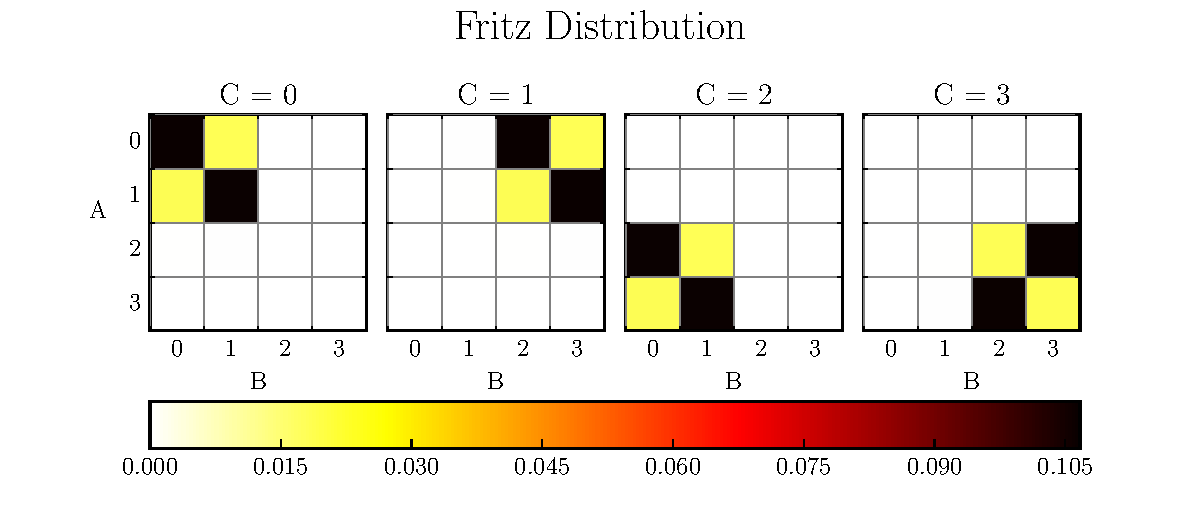
\includegraphics[width=\linewidth]{../../figures/distributions/fritz_dist_plot_brazil.pdf}
    \end{center}
    \[ \probplotvalue{253, 253, 84} = \f{1}{32}\br{2 - \sqrt{2}} \qquad \probplotvalue{11, 1, 0} = \f{1}{32}\br{2 + \sqrt{2}}\]
\end{frame}

\begin{frame}
    \frametitle{Maximal Violation}
    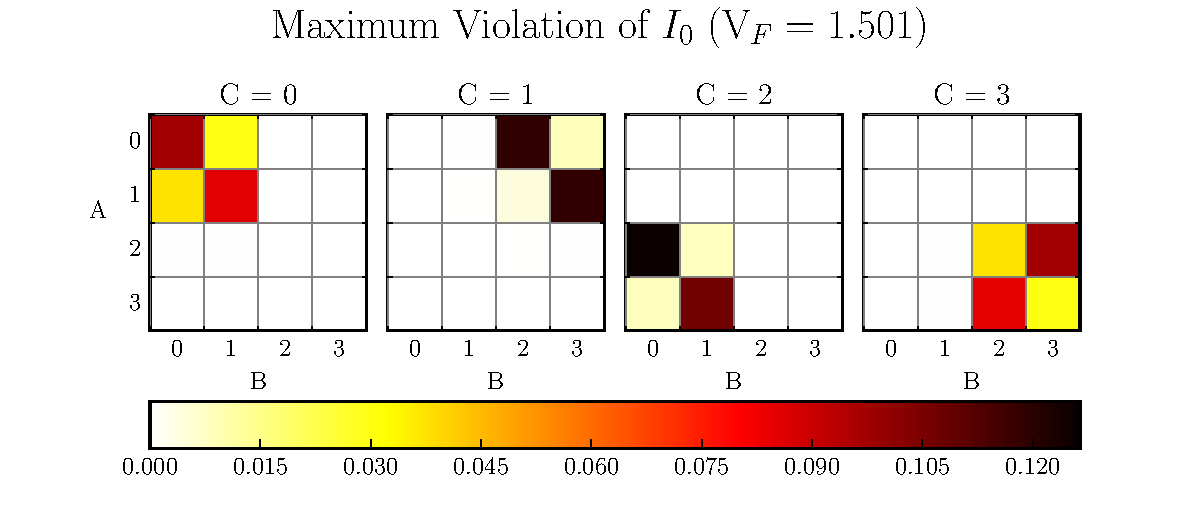
\includegraphics[width=\linewidth]{../../figures/distributions/plotted_dist_I_0_max_violation.pdf}
    \[ \text{Relative Violation:} \qquad V_F = \f{\min_P\bc{I\br{P}}}{I\br{P_F}} \]
\end{frame}

\begin{frame}
    \frametitle{Maximal Violation Symmetric}
    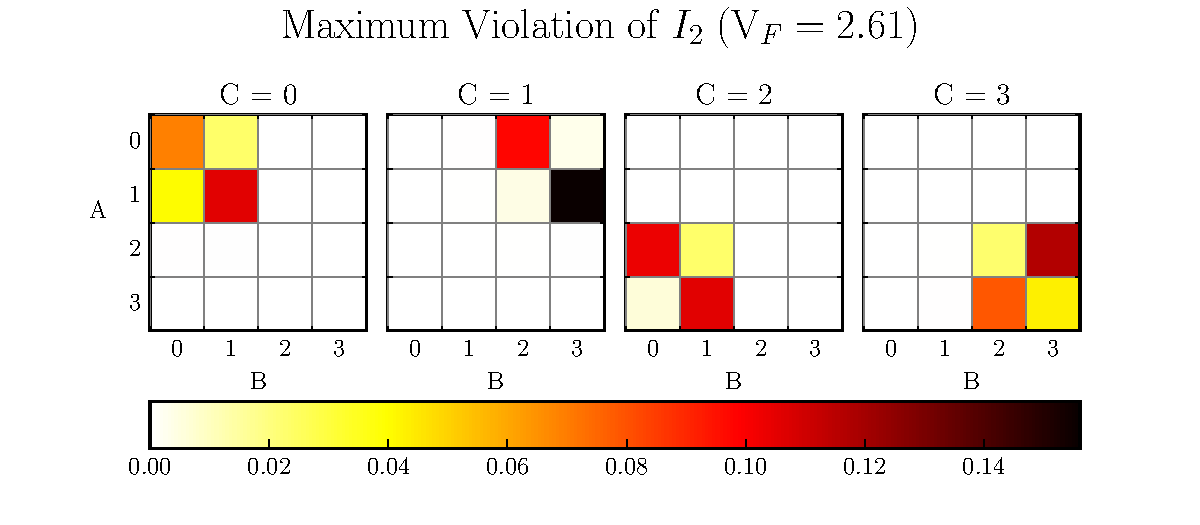
\includegraphics[width=\linewidth]{../../figures/distributions/plotted_dist_I_2_max_violation.pdf}
    \[ \text{Relative Violation:} \qquad V_F = \f{\min_P\bc{I\br{P}}}{I\br{P_F}} \]
\end{frame}

\begin{frame}
    \frametitle{Uniform Noise}
    \[ \s{U}_{\varepsilon}\br{P} = \br{1 - \varepsilon} P + \varepsilon \s{U} \]
    \begin{center}
        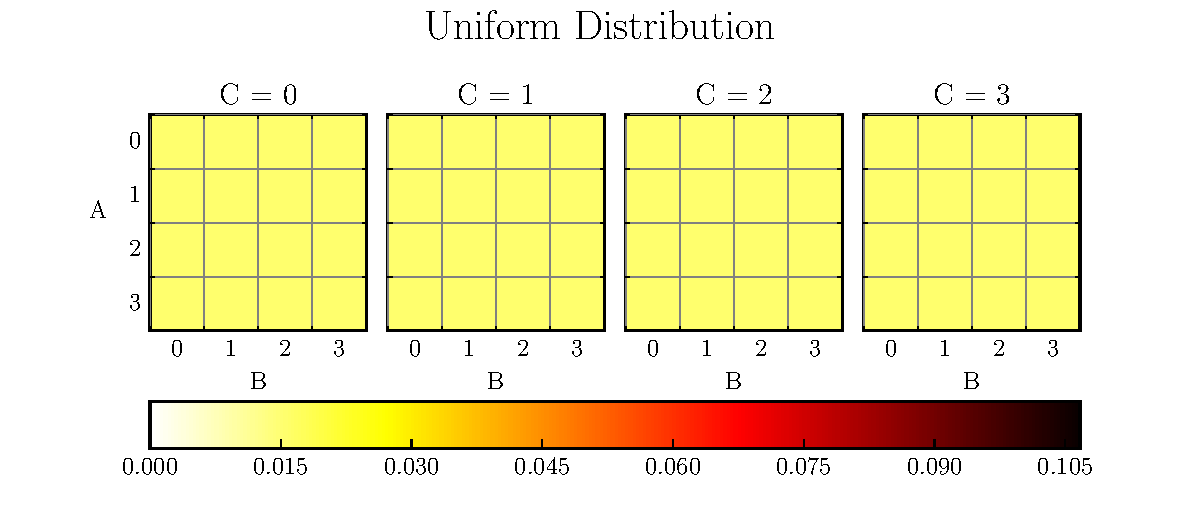
\includegraphics[width=\linewidth]{../../figures/distributions/uniform_dist_plot.pdf}
    \end{center}
    \[ \probplotvalue{255, 255, 109} = \f{1}{64} \]
    % \begin{center}
    %     \begin{tikzpicture}
    %         \pgfmathsetmacro{\ts}{0.5}; % term spacing
    %         \draw[] (0*\ts,0) node[]{$P_\varepsilon$};
    %         \draw[] (1*\ts,0) node[]{$=$};
    %         \draw[] (2*\ts,0) node[]{$(1-\varepsilon)P_{F}$};
    %         \draw[] (3*\ts,0) node[]{$+$};
    %         \draw[] (4*\ts,0) node[]{$\delta$};
    %     \end{tikzpicture}
    % \end{center}
\end{frame}

\begin{frame}
    \frametitle{Robust to Noise Zoomed}
    \begin{center}
        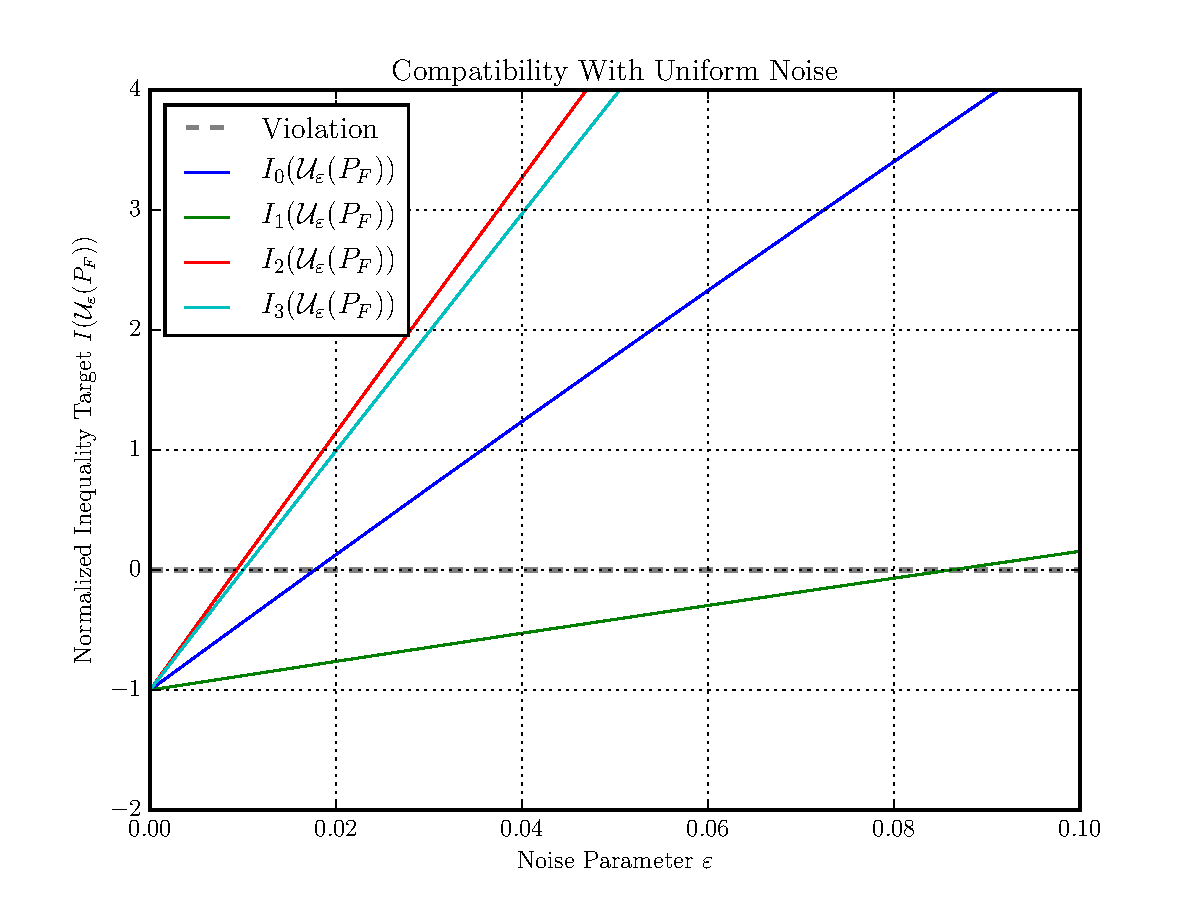
\includegraphics[width=\linewidth]{../../figures/noise/four_rep_inequalities_uniform_noise_zoomed.pdf}
    \end{center}
\end{frame}

\begin{frame}
    \frametitle{Conclusions}
    \begin{itemize}
        \item Quantum/Classical difference can be observed in the triangle scenario
        \item Successful demonstration of the inflation technique
        \item Developed new algorithmic tools to find such inequalities
        \item New measures of non-classicality which lead to new quantum mechanical resources
    \end{itemize}
\end{frame}

\begin{frame}[allowframebreaks]
    \frametitle{References}
    \printbibliography
\end{frame}

\section{Appendix A: Optional Slides}

\begin{frame}
    \frametitle{Notation}
    \textbf{Question:} Which marginal models $\prob^{\mscenario}$ are \term{compatible} with a causal structure $\graph$?\\
    \begin{itemize}
        \item \term{Marginal model} $\prob^{\mscenario}$ is collection of probability distributions
        \[ \prob^{\mscenario} = \bc{\prob[V_1], \ldots, \prob[V_k]} \]
        \item \term{Marginal scenario} $\mscenario = \bc{V_1, \ldots, V_k}$
        \[ V \in \mscenario, V' \subseteq V  \implies V' \in \mscenario \]
        % \item Marginal scenario forms a \textit{simplicial complex}
        % \[ V \in \mscenario, V' \subseteq V  \implies V' \in \mscenario \]
        \item \term{Joint random variables} $\jointvar = {\bigcup}_{i} V_i = \bc{v_1, \ldots, v_n}$
        \item \term{Causal Structure} $\graph = \br{\nodes, \edges}$ is a directed acyclic graph (DAG)
        \item Nodes classified into \term{latent nodes} $\nodes_{L}$ and \term{observed nodes} $\nodes_{O}$
    \end{itemize}
    \note[item]{Before continuing, I will define exactly what I mean by causal compatibility}
    \note[item]{Causal compatibility refers to the compatibility between causal structures and marginal models}
    \note[item]{Marginal model is collection of probability distributions over sets of random variables}
    \note[item]{Marginal scenario refers to the those sets of random variables}
    \note[item]{The complete set of random variables are the joint random variables}
\end{frame}

\begin{frame}
    \frametitle{Graph Theory}
    Let $n, m \in \nodes$ be nodes of the graph $\graph$.
    \begin{itemize}
        \item \term{parents of $n$}: $\Pa[\graph]{n} \defined \bc{m \mid m \to n}$
        \item \term{children of $n$}: $\Ch[\graph]{n} \defined \bc{m \mid n \to m}$
        \item \term{ancestry of $n$}: $\An[\graph]{n} \defined \bigcup_{i\in\mathbb{W}} \Pa[\graph][i]{n}$
        \[ \Pa[\graph][0]{n} = n \qquad \Pa[\graph][i]{n} \defined \Pa[\graph]{\Pa[\graph][i-1]{n}} \]
    \end{itemize}
    Notation extends to sets of nodes $N \subseteq \nodes$,
    \begin{itemize}
        \item \term{parents of $N$}: $\Pa[\graph]{N} \defined \bigcup_{n\in N}\Pa[\graph]{n}$
        \item \term{children of $N$}: $\Ch[\graph]{N} \defined \bigcup_{n\in N}\Ch[\graph]{n}$
        \item \term{ancestry of $N$}: $\An[\graph]{N} \defined \bigcup_{n\in N}\An[\graph]{n}$
    \end{itemize}
    An \term{induced subgraph} of $\graph = \br{\nodes, \edges}$ due to $N \subseteq \nodes$
    \[ \Sub[\graph]{N} = \br{N, \bc{e \in \edges \mid e \subseteq N}} \]
\end{frame}

\begin{frame}
    \frametitle{Causal Compatibility}
    \textbf{Question:} Which marginal models $\prob^{\mscenario}$ are \term{compatible} with a causal structure $\graph$?\\
    \textbf{Answer:} $\prob^{\mscenario}$ is compatible with $\graph$ if there exists a set of \term{casual parameters}
    \[ \bc{\prob[n \mid \Pa[\graph]{n}] \mid n \in \nodes} \]
    Such that for each $V \in \mscenario$, $\prob[V]$ can be recovered:
    \begin{enumerate}
        \item $\prob[\nodes] = \prod_{n\in\nodes}\prob[n \mid \Pa[\graph]{n}]$
        \item $\prob[V] = \sum_{\nodes \setminus V} \prob[\nodes]$
    \end{enumerate}
    \textbf{Inequality:} A \term{casual compatibility inequality} $I$ is an inequality over $\prob^{\mscenario}$ that is satisfied by all compatible $\prob^{\mscenario}$
\end{frame}

\begin{frame}
    \frametitle{Deriving Inequalities}
    Two necessary components to compatibility:
    \begin{enumerate}
        \item \term{Marginal problem}: $\forall V \in \mscenario : \prob[V] = \sum_{\nodes \setminus V} \prob[\nodes]$
        \begin{itemize}
            \item Is the marginal model contextual or non-contextual?
            \item 3 distinct ways to tackle this problem
            \begin{enumerate}
                \item Convex hull, Polytope projection, Fourier-Motzkin
                \item Possibilistic Hardy Inequalities (Hypergraph transversals)
                \item Linear Program Feasibility/Infeasibility
            \end{enumerate}
        \end{itemize}
        \item \term{Markov Separation}: $\prob[\nodes] = \prod_{n\in\nodes}\prob[n \mid \Pa[\graph]{n}]$
        \begin{itemize}
            \item Much harder to determine since latent nodes $\nodes_O$ have unspecified behaviour
            \item It is possible to turn Markov Separation problem into a Marginal problem (at least partially)
        \end{itemize}
    \end{enumerate}
\end{frame}

\begin{frame}
    \frametitle{Inflation Technique}
    Developed by Wolfe, Spekkens, and Fritz \cite{Inflation}
    \begin{definition}
        An \term{inflation} of a causal structure $\graph$ is another causal structure $\graph'$ such that:
        \[ \forall n' \in \nodes', n' \sim n \in \nodes: \AnSub[\graph']{n'} \sim \AnSub[\graph]{n} \]
        Where $\AnSub[\graph]{n}$ denotes the ancestral sub-graph of $n$ in $\graph$
        \[ \AnSub[\graph]{n} = \Sub[\graph]{\An[\graph]{n}} \]
        And '$\sim$' is a \term{copy-index} equivalence relation
        \[ A_1 \sim A_2 \sim A \not \sim B_1 \sim B_2 \sim B \]
    \end{definition}
\end{frame}

\begin{frame}
    \frametitle{Inflation Lemma}
    If one has obtained $\graph$, inflation $\graph'$ and \textit{compatible} marginal distribution $\prob[N]$ where $N \subseteq \nodes$, then:
    \begin{enumerate}
        \item There exists causal parameters $\bc{\prob[n\mid\Pa[\graph]{n}] \mid n \in \nodes}$ such that
        \[ \prob[N] = \prod_{n \in N}\prob[n\mid\Pa[\graph]{n}] \]
        \item $\AnSub[\graph']{n'} \sim \AnSub[\graph]{n} \implies \Pa[\graph']{n'} \sim \Pa[\graph]{n}$
        \item Construct \term{inflated causal parameters}
        \[ \forall n' \in \nodes' : \prob[n'\mid\Pa[\graph']{n'}] \defined \prob[n\mid\Pa[\graph]{n}]\]
        \item Obtain \textit{compatible} marginal distributions over any $N' \subseteq \nodes'$
        \[ \prob[N'] = \prod_{n' \in N'}\prob[n'\mid\Pa[\graph']{n'}] \]
    \end{enumerate}
\end{frame}

\begin{frame}
    \frametitle{Inflation Lemma Cont'd}
    \begin{itemize}
        \item Inflation procedure holds for any $N \in \nodes, N' \in \nodes'$ where $\AnSub[\graph]{N} \sim \AnSub[\graph']{N'}$
        \item Define \term{injectable sets of $\graph'$} and \term{images of the injectable of $\graph$}
    \end{itemize}
    \begin{align*}
        \Inj[\graph]{\graph'} &\defined \bc{N' \subseteq \nodes' \mid \exists N \subseteq \nodes : \AnSub[\graph]{N} \sim \AnSub[\graph']{N'}} \\
        \ImInj[\graph]{\graph'} &\defined \bc{N \subseteq \nodes \mid \exists N' \subseteq \nodes' : \AnSub[\graph]{N} \sim \AnSub[\graph']{N'}}
    \end{align*}
    \begin{itemize}
        \item For $N' \in \Inj[\graph]{\graph'}$ there is a \textit{unique} $N \subseteq \nodes$ such that $\AnSub[\graph]{N} \sim \AnSub[\graph']{N'}$
        \item For $N \in \Inj[\graph]{\graph}$ there can \textit{exist many} $N' \subseteq \nodes'$ such that $\AnSub[\graph]{N} \sim \AnSub[\graph']{N'}$
    \end{itemize}
\end{frame}

\begin{frame}
    \frametitle{Inflation Lemma Cont'd}
    \begin{lemma}
        \term{The Inflation Lemma:}~\cite[lemma 3]{Inflation} Given a particular inflation $\graph'$ of $\graph$, if a marginal model $\bc{\prob[N] \mid N \in \ImInj[\graph]{\graph'}}$ is compatible with $\graph$ then all marginal models $\bc{\prob[N'] \mid N' \in \Inj[\graph]{\graph'}}$ are compatible with $\graph'$ provided that $\prob[N] = \prob[N']$ for all instances where $N \sim N'$.
    \end{lemma}
    \begin{corollary}
        Any causal compatibility inequality $I'$ constraining the injectable sets $\Inj[\graph]{\graph'}$ can be \term{deflated} into a causal compatibility inequality $I$ constraining the images of the injectable sets $\ImInj[\graph]{\graph'}$.
    \end{corollary}
\end{frame}

\begin{frame}
    \frametitle{Pre-injectable Sets}
    \begin{itemize}
        \item $d$-separation relations $+$ inflation $=$ polynomial inequalities over $\graph$
        \item Restrict focus to sets $N'$ that are partitioned into $N_1', N_2'$ $d$-separated by empty set $\emptyset$
        \item A \term{pre-injectable set} $N'$:
        \[ N' = {\coprod}_i N_i' \quad \forall i: N_i' \in \Inj[\graph]{\graph'} \]
        \[ \forall i, j : N_i' \ancestralindep N_j' \iff \An[\graph']{N'_i} \cap \An[\graph']{N'_j} = \emptyset \]
        \item Only need to consider \term{maximal pre-injectable sets} $\PreInj[\graph]{\graph'}$
    \end{itemize}
\end{frame}

\begin{frame}
    \frametitle{Network Permutation Matrix}
    \begin{columns}
        \column{0.6\linewidth}
        \begin{itemize}
            \item States and measurements in the Triangle Scenario are not aligned
            \item Without $\netperm$, $\prob[ABC]$ would be separable
            \item Required to align $B$'s measurement over $\Tr_{A,C}\br{\rho_{AB} \otimes \rho_{BC}}$
            \item $\netperm$ is a $2^6 \times 2^6$ matrix
            \item Shifts one qubit to the left
        \end{itemize}
        \column{0.4\linewidth}
            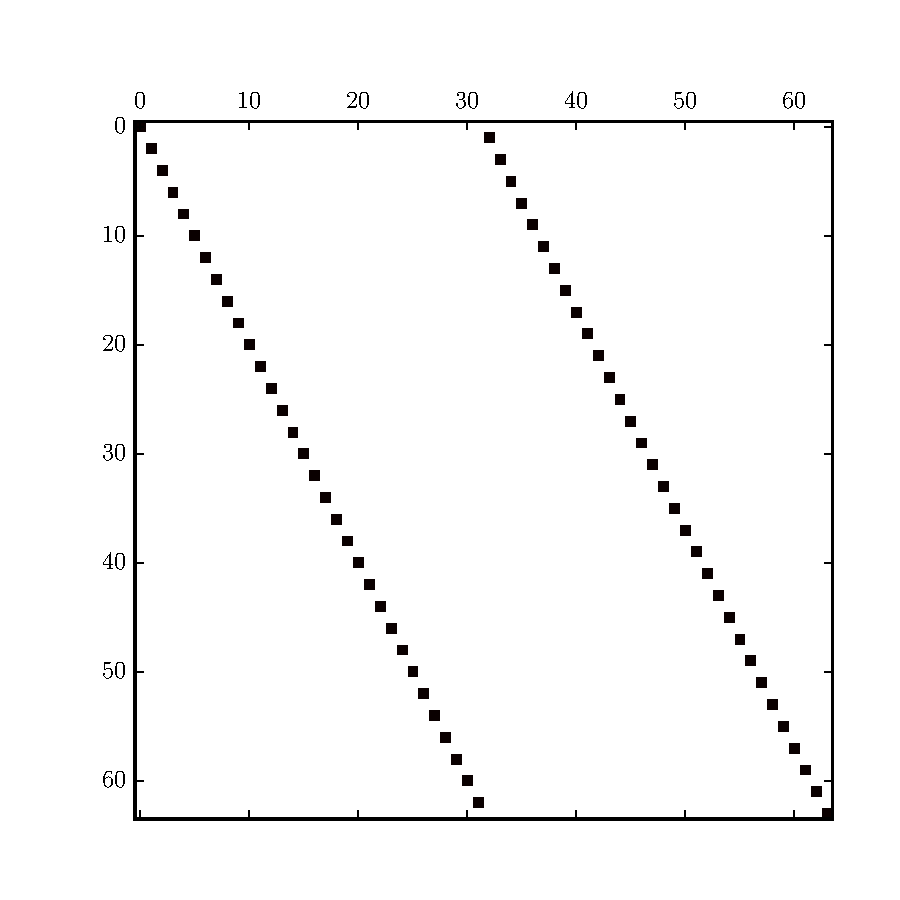
\includegraphics[trim={1.0cm 1.2cm 1.0cm 1cm},clip,width=1.0\textwidth]{../../figures/perm_mtrx.pdf}
    \end{columns}
    \[ \netperm \defined \sum_{\ket{q_i} \in \bc{\ket{0}, \ket{1}}}\ket{q_2q_3q_4q_5q_6q_1}\bra{q_1q_2q_3q_4q_5q_6} \]
\end{frame}

\begin{frame}
    \frametitle{Outcomes and Events}
    \begin{definition}
        Each variable $v$ has finite set of \term{outcomes} $O_v$. \\
        Each set of variables $V$ has finite set of \term{events} $\Events{V}$:
        \[ \Events{V} \defined \bc{s: V \to O_V \mid \forall v \in V, s\br{v} \in O_v} \]
    \end{definition}
    \begin{definition}
        The set of events over the joint variables $\Events{\jointvar}$ are termed the \term{joint events}.
    \end{definition}
    \begin{definition}
        The set of events over the marginal contexts are the \term{marginal events}
        \[ \Events{\mscenario} \defined \coprod_{V \in \mscenario} \Events{V} \]
    \end{definition}
\end{frame}

\begin{frame}
    \frametitle{Distribution Vectors}
    \begin{definition}
        The \term{joint distribution vector} $\probvec^{\jointvar}$
        \[ \probvec^{\jointvar}_j = \prob[\jointvar][j] \quad \forall j \in \Events{\jointvar}\]
    \end{definition}
    \begin{definition}
        The \term{marginal distribution vector} $\probvec^{\mscenario}$
        \[ \probvec^{\mscenario}_m = \prob[\Dom{m}][m] \quad \forall m \in \Events{\mscenario}, \Dom{m} \in \mscenario\]
    \end{definition}
    Can now write complete marginal problem as matrix multiplication:
    \[ \forall V \in \mscenario : \prob[V] = \sum_{\jointvar \setminus V} \prob[\jointvar] \iff \probvec^{\mscenario} = M \tcdot \probvec^{\jointvar} \]
\end{frame}

\begin{frame}
    \frametitle{Incidence Matrix}
    \begin{itemize}
        \item \term{Incidence matrix} $M$ is a bit-wise matrix
        \item Row-indexed by marginal events $m \in \Events{\mscenario}$
        \item Column-indexed by joint events $j \in \Events{\jointvar}$
        \[ M_{m,j} = \begin{cases}
            1 & m = j|_{\Dom{m}} \\
            0 & \text{otherwise}
        \end{cases} \]
        \begin{gather*}
        \# \text{Columns} = \abs{\Events{\jointvar}} = \prod_{v \in \jointvar} \abs{O_{v}} \\
        \# \text{Rows} = \abs{\Events{\mscenario}} = \sum_{V \in \mscenario} \prod_{v \in V} \abs{O_{v}}
        \end{gather*}

    \end{itemize}
\end{frame}


\begin{frame}
    \frametitle{Causal Symmetry}
    \begin{itemize}
        \item Desirable to find compatibility inequality $I$ such that
        \[ \forall \varphi \in \Perm{A,B,C} : \varphi\bs{I} = I \]
        \item Compatibility is independent of variable labels $I, \graph \to \varphi\bs{I}, \varphi\bs{\graph}$
        \item Need $\varphi\bs{\graph} = \graph$ to find new $\varphi\bs{I}$
    \end{itemize}
    \begin{definition}
        The \term{causal symmetry group} of causal structure $\graph$:
        \[ \Aut{\graph} = \bc{\varphi \in \Perm{\nodes} \mid \varphi\bs{\graph} = \graph} \]
        Strictly speaking, one needs to preserve observable nodes:
        \[ \Aut[\nodes_O]{\graph} = \bc{\varphi \in \Aut{\graph} \mid \varphi\bs{\nodes_O} = \nodes_O} \]
    \end{definition}
    \note<1>[item]{Fritz distribution is incompatible with Triangle scenario because party $C$ plays the role of measurement settings for both $A$ and $B$}
    \note<1>[item]{In order to find quantum distributions different from $P_F$ in the Triangle Scenario, it is therefore desirable to find a proof of its incompatibility (i.e. inequality) that is symmetric under exchange of parties}
    \note<1>[item]{Surprisingly, it is possible to do so!}
    \note<1>[item]{Here is how.}
    \note<1>[item]{First, we will formally define the symmetry group in question}
    \note<1>[item]{Causal symmetry group is the group of automorphisms on causal structure}
\end{frame}

\begin{frame}
    \frametitle{Causal Symmetry and Inflation}
    \begin{itemize}
        \item Causal symmetry group for $\graph'$ is no good!
        \item Not possible to deflate inequality if it's not in terms of injectable sets
        \begin{definition}
            The \term{restricted causal symmetry group} $\Phi$ of $\graph'$:
            \[ \Phi = \Aut[\PreInj[\graph]{\graph'}]{\graph'} \]
        \end{definition}
    \end{itemize}
\end{frame}

\begin{frame}
    \frametitle{Restricted Causal Symmetry of Large Inflation}
    \begin{itemize}
        \item $\Phi$ for the large inflation is an order $48$ group with $4$ generators
    \end{itemize}
    \begin{equation*}
    \begin{aligned}[c]
    &\hspace{1mm}\gep_1 \\
    A_1 &\to A_4 \\A_2 &\to A_3 \\A_3 &\to A_2 \\A_4 &\to A_1 \\B_1 &\to B_4 \\B_2 &\to B_3 \\B_3 &\to B_2 \\B_4 &\to B_1 \\C_1 &\to C_4 \\C_2 &\to C_3 \\C_3 &\to C_2 \\C_4 &\to C_1
    \end{aligned}
    \quad
    \begin{aligned}[c]
    &\hspace{1mm}\gep_2 \\
    A_1 &\to A_1 \\A_2 &\to A_3 \\A_3 &\to A_2 \\A_4 &\to A_4 \\B_1 &\to C_1 \\B_2 &\to C_3 \\B_3 &\to C_2 \\B_4 &\to C_4 \\C_1 &\to B_1 \\C_2 &\to B_3 \\C_3 &\to B_2 \\C_4 &\to B_4
    \end{aligned}
    \quad
    \begin{aligned}[c]
    &\hspace{1mm}\gep_3 \\
    A_1 &\to C_1 \\A_2 &\to C_2 \\A_3 &\to C_3 \\A_4 &\to C_4 \\B_1 &\to A_1 \\B_2 &\to A_2 \\B_3 &\to A_3 \\B_4 &\to A_4 \\C_1 &\to B_1 \\C_2 &\to B_2 \\C_3 &\to B_3 \\C_4 &\to B_4
    \end{aligned}
    \quad
    \begin{aligned}[c]
    &\hspace{1mm}\gep_4 \\
    A_1 &\to A_1 \\A_2 &\to A_2 \\A_3 &\to A_3 \\A_4 &\to A_4 \\B_1 &\to B_2 \\B_2 &\to B_1 \\B_3 &\to B_4 \\B_4 &\to B_3 \\C_1 &\to C_3 \\C_2 &\to C_4 \\C_3 &\to C_1 \\C_4 &\to C_2
    \end{aligned}
    \end{equation*}
\end{frame}

\begin{frame}
    \frametitle{Symmetric Incidence}
    \begin{itemize}
        \item Group orbits through repeated action of $\varphi \in \Phi$ on $m \in \Events{\mscenario}$ and $j \in \Events{\jointvar}$
    \end{itemize}
    \begin{align*}
        \Phi\bs{m} &\defined \bc{\varphi\bs{m} \mid \varphi \in \Phi} \\
        \Phi\bs{j} &\defined \bc{\varphi\bs{j} \mid \varphi \in \Phi}
    \end{align*}
    \begin{itemize}
        \item Construct \term{symmetric incidence matrix} $\Phi\bs{M}$
    \end{itemize}
    \[ \Phi\bs{M}_{\Phi\bs{m}, \Phi\bs{j}} = \sum_{m' \in \Phi\bs{m}}\sum_{j' \in \Phi\bs{j}} M_{m',j'} \]
    \[ \Phi\bs{M} = \La_{\Phi\bs{\Events{\mscenario}}}\tcdot M \tcdot \La_{\Phi\bs{\Events{\jointvar}}} \]
    \begin{itemize}
        \item $\Phi\bs{M}$ not a bit-wise matrix like $M$
        \item For large inflation $M$ is $16,896 \times 16,777,216$
        \item For large inflation $\Phi\bs{M}$ is $450 \times 358,120$ % 3566922 entries
    \end{itemize}
\end{frame}


\begin{frame}
    \frametitle{Symmetric Inequalities}
    \begin{itemize}
        \item Certificate inequalities are curated/constructed to witness violation of particular distribution
        \item Above inequality not the best candidate to search for non-locality different than Fritz distribution
        \item Perhaps one could obtain inequality that does not assign special preference to $C$
        \item Desirable to find compatibility inequality $I$ such that
        \[ \forall \varphi \in \Perm{A,B,C} : \varphi\bs{I} = I \]
    \end{itemize}
\end{frame}


\begin{frame}
    \frametitle{Symmetrized Fritz}
    \begin{center}
        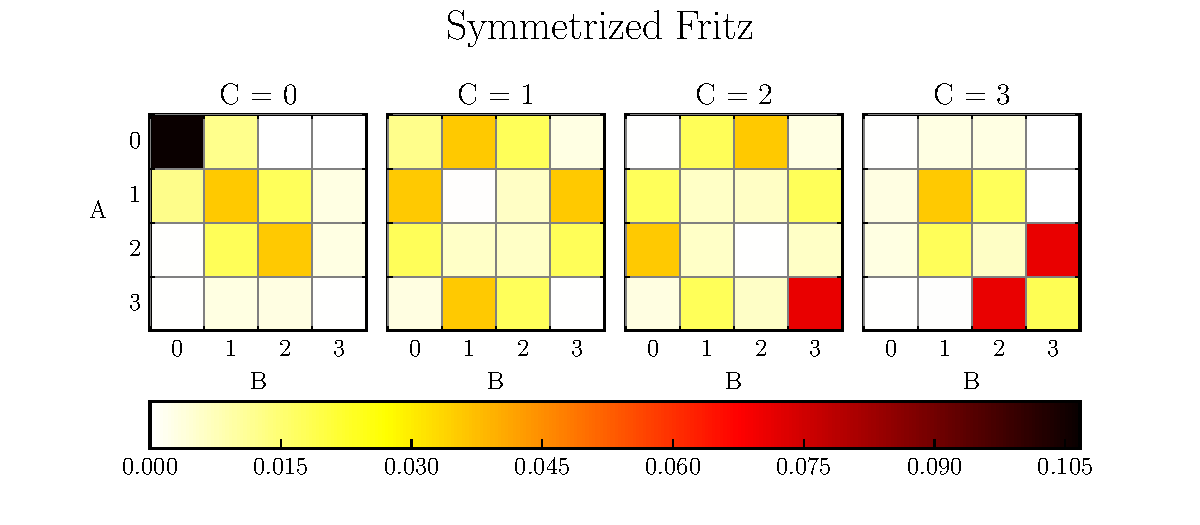
\includegraphics[width=\linewidth]{../../figures/distributions/symmetrized_fritz.pdf}
    \end{center}
    \begin{itemize}
        \item More non-local yet not quantum-accessible
        \item Quantum-accessible distributions form non-context set
    \end{itemize}
\end{frame}

\begin{frame}
    \frametitle{Parameterizing POVMs}
    \begin{itemize}
        \item Each party $\br{A, B, C}$ is assigned a \term{projective-operator valued measure (POVM)} $\br{M_A, M_B, M_C}$
        \[ \forall \ket{\psi} \in \Hilb^d : \bra{\psi} M_\chi \ket{\psi} \geq 0 \quad M_\chi = M_\chi^{\dagger} \]
        \item $n$-outcome measurement
        \[ M_\chi = \bc{M_{\chi, 1}, \ldots, M_{\chi, n}} \quad \sum_{i=1}^{n} M_{\chi, i} = \ident \]
        \item For $n = 2$ outcomes, a parameterization exists by constraining the eigenvalues of $M_{\chi, i}$; for $n > 2$ not aware of anything
        \item Warrants consideration of \term{projective-valued measures (PVMs)}
    \end{itemize}
    \note<1>[item]{Naimark's Dilation Theorem}
\end{frame}

\begin{frame}
    \frametitle{Cholesky Parameterization of States}
    \begin{itemize}
        \item Each latent resource $\rho \in \br{\rho_{AB}, \rho_{BC}, \rho_{CA}}$ modeled as bipartite qubit state acting on $\Hilb^{d/2} \otimes \Hilb^{d/2}$
        \item $d \times d$ positive semi-definite (PSD) hermitian matrices with unitary trace
        \item \term{Cholesky Parametrization} allows one to write any hermitian PSD as $\rho = T^{\dagger} T$
        \item For $d = 4$:
        \[ T = \begin{bmatrix}\la_{1}&0&0&0\\\la_{2} + i \la_{3}&\la_{4}&0&0\\\la_{5} + i \la_{6}&\la_{7} + i \la_{8}&\la_{9}&0\\\la_{10} + i \la_{11}&\la_{12} + i \la_{13}&\la_{14} + i \la_{15}&\la_{16}\end{bmatrix} \]
        \item $d^2$ real-valued parameters
        \item Normalized $\rho = {T^{\dagger}T}/{\Tr\br{T^{\dagger} T}}$ adds degeneracy
    \end{itemize}
\end{frame}

\section{Appendix B: Local Minima Concerns}

\begin{frame}
    \frametitle{Results}
    \begin{itemize}
        \item Finding global minimum is tricky
        \item Difficult to converge to violation
        \item Noisy seed (Gaussian noise):
        \[ \la_{(0)} = \la_{(F)} + \de \la \qquad \de \la_{i} \sim \s{N}\br{\mu = 0, \si^2 = (2\pi10^{\chi})^2} \]
        \item Uniform seed:
        \[ \la_{(0), i} \sim \s{U}\br{[0, 2\pi]} \]
    \end{itemize}
\end{frame}

\begin{frame}
    \frametitle{Fritz Local Minima}
    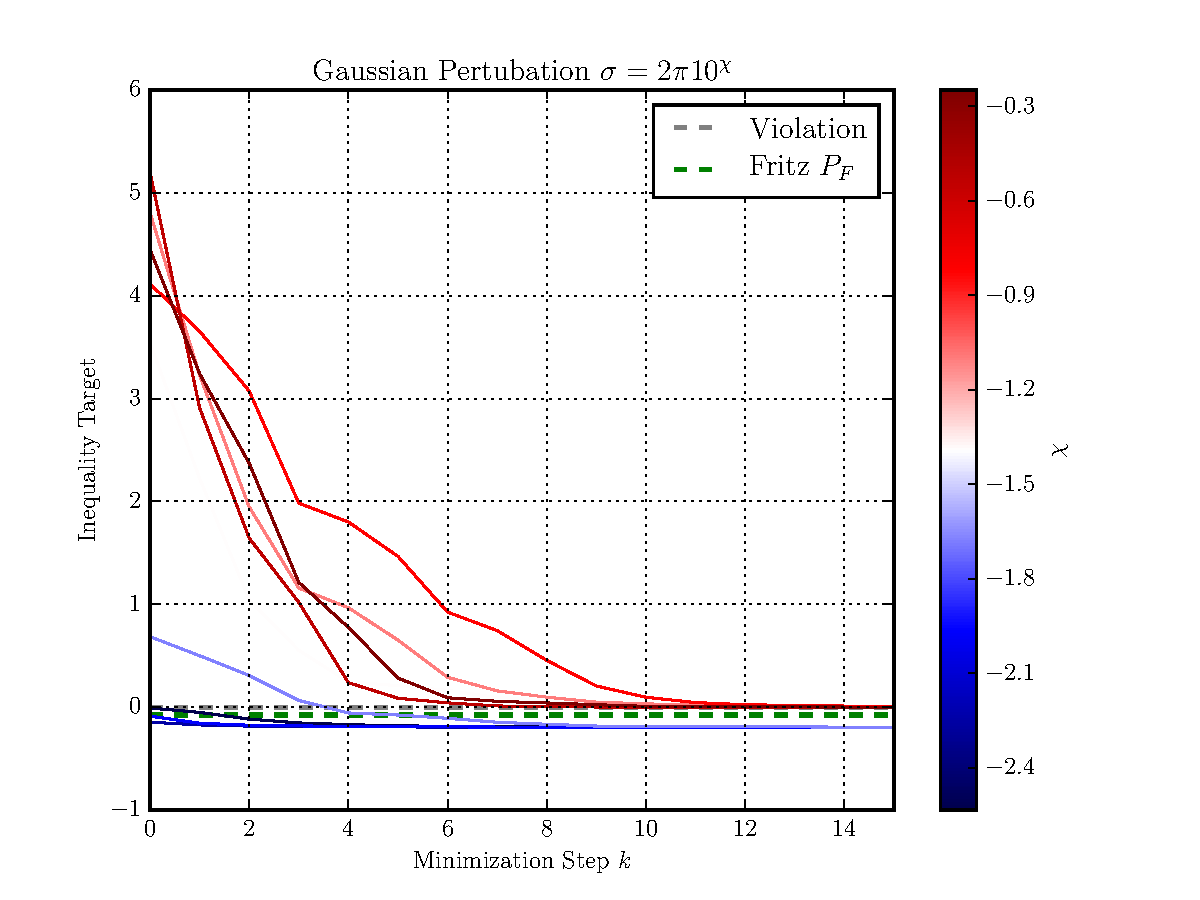
\includegraphics[width=\linewidth]{../../figures/optimizations/Gaussian_Perturbation_Fritz_Color_Default.pdf}
\end{frame}

\begin{frame}
    \frametitle{Fritz Local Minima Zoomed}
    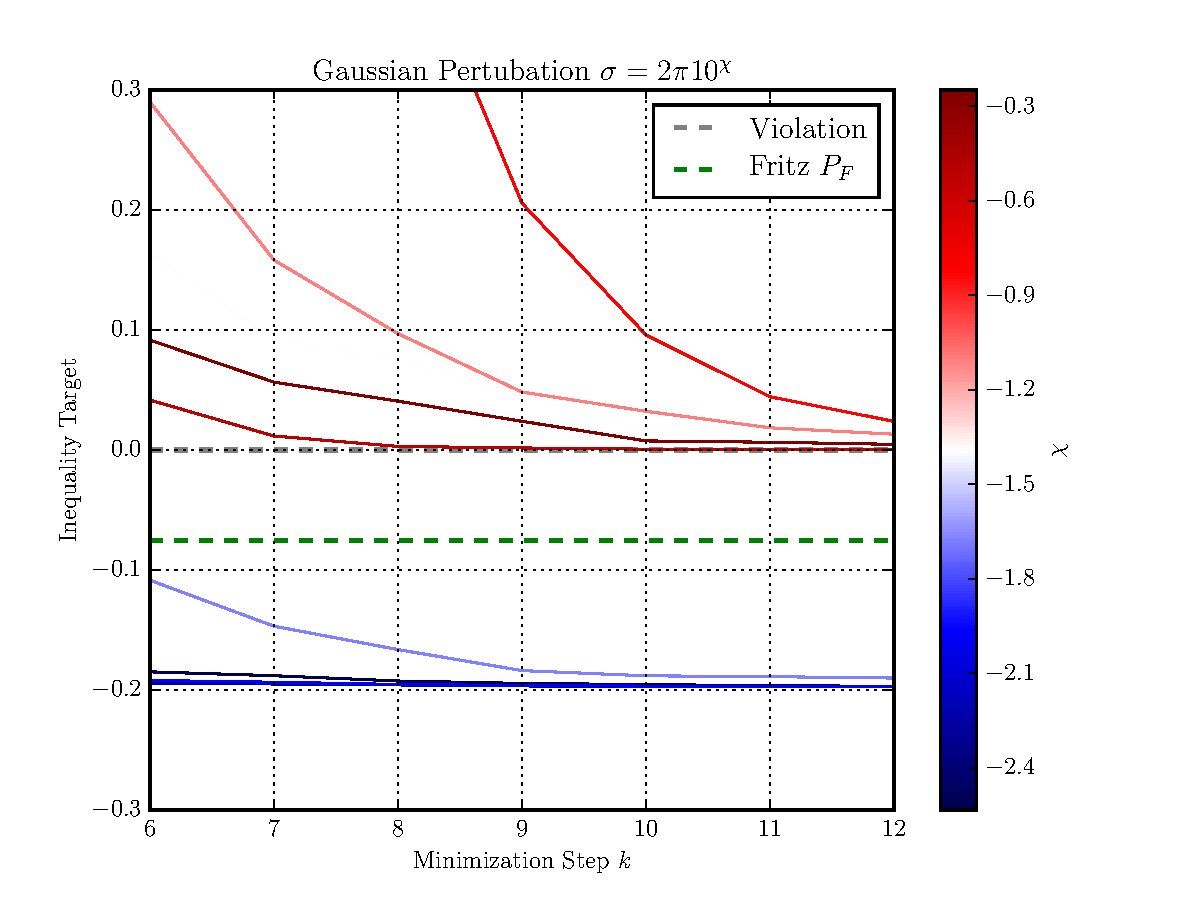
\includegraphics[width=\linewidth]{../../figures/optimizations/Gaussian_Perturbation_Fritz_Color_Zoomed.pdf}
\end{frame}

\begin{frame}
    \frametitle{Max Entangled vs. Max Violating (???)}
    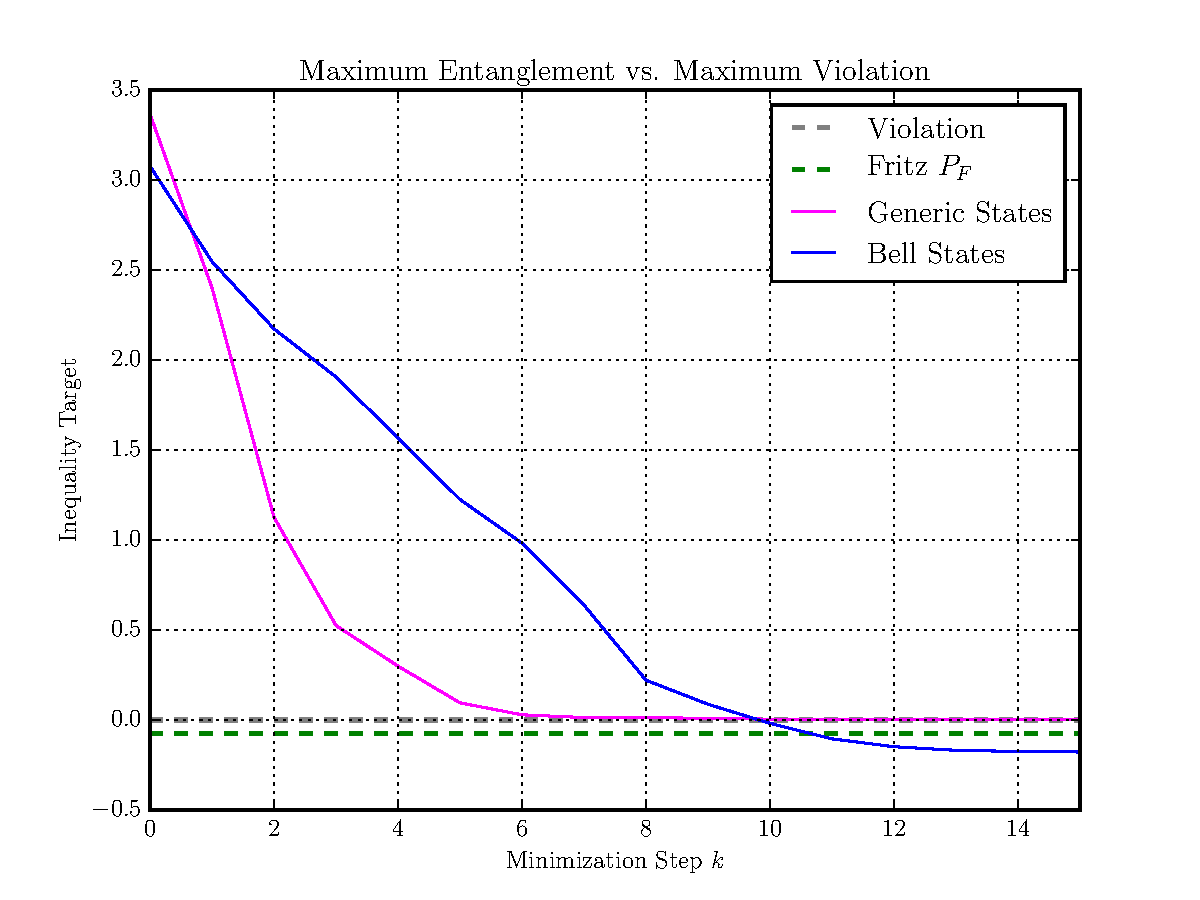
\includegraphics[width=\linewidth]{../../figures/optimizations/Max_Entanglement_vs_Max_Violation_random_seed.pdf}
\end{frame}

\begin{frame}
    \frametitle{Max Entangled vs. Max Violating (???)}
    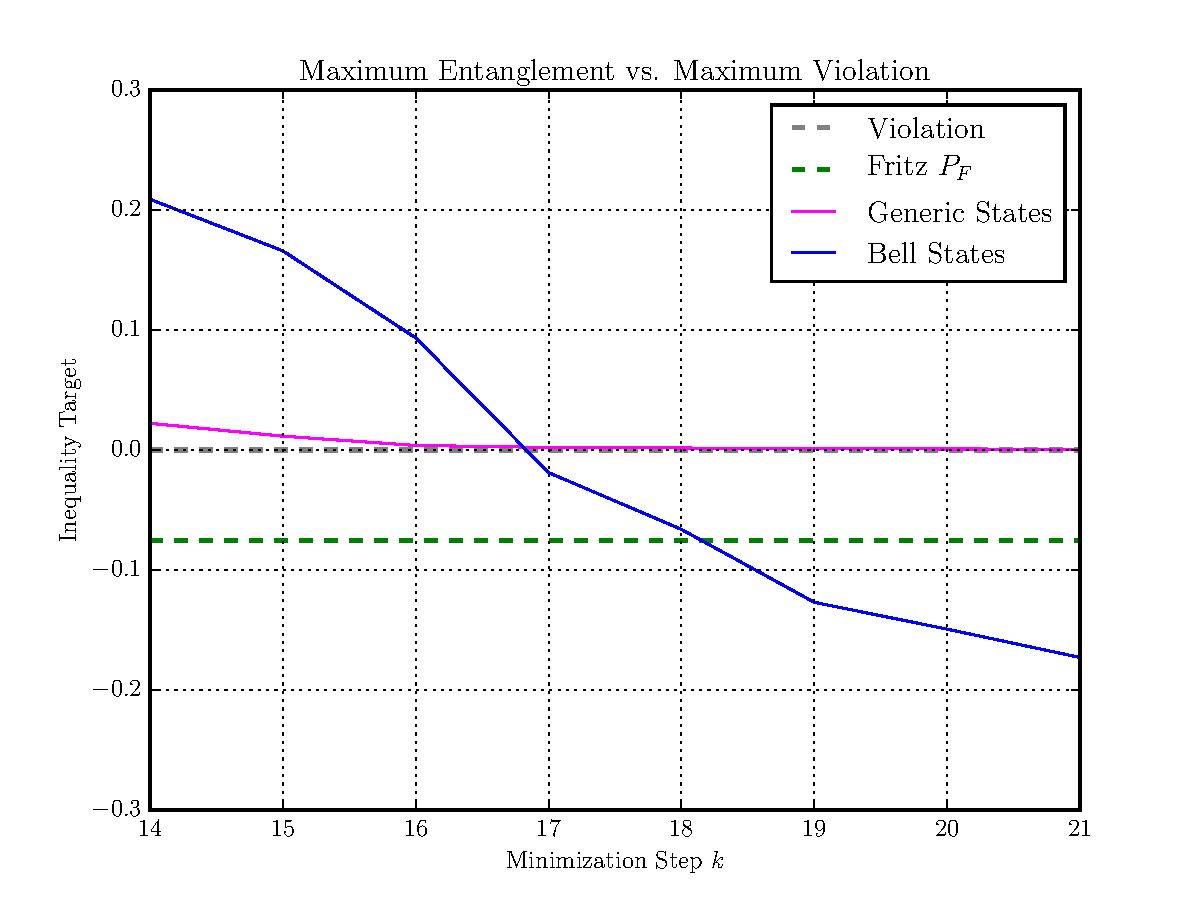
\includegraphics[width=\linewidth]{../../figures/optimizations/Max_Entanglement_vs_Max_Violation_random_seed_Zoomed.pdf}
\end{frame}


\section{Section C: Inflation Technique}
\begin{frame}
    \frametitle{Demonstrating Inflation Technique}
    \vfill
    \begin{center}
    \begin{columns}
        \column{0.5\linewidth}%
        \scalebox{1.0}{\begin{tikzpicture}[scale=1]
    \begin{scope}[every node/.style=observed, onslide=<2->{fade}]
        \node[onslide=<3>{unfade}] (C) at (-2, 0) {$\p{C}$};
        \node (B) at (2, 0) {$\p{B}$};
        \node[onslide=<2>{unfade}] (A) at (0, {2*sqrt(3)}) {$\p{A}$};
    \end{scope}
    \begin{scope}[every node/.style=latent, onslide=<2->{fade}]
        \node[onslide=<2-3>{unfade}] (X) at (-1, {sqrt(3)}) {$\p{X}$};
        \node[onslide=<2>{unfade}] (Y) at (1, {sqrt(3)}) {$\p{Y}$};
        \node[onslide=<3>{unfade}] (Z) at (0, 0) {$\p{Z}$};
    \end{scope}
    \begin{scope}[every path/.style={draw=cause, thick}, onslide=<2->{fade}]
        \path[postaction={on each segment={mid arrow}}]
        (Y) -- (B)
        (Z) -- (B)
        ;
        \path[postaction={on each segment={mid arrow}}, onslide=<3>{unfade}]
        (X) -- (C)
        (Z) -- (C)
        ;
        \path[postaction={on each segment={mid arrow}}, onslide=<2>{unfade}]
        (X) -- (A)
        (Y) -- (A)
        ;
    \end{scope}
\end{tikzpicture}}
        \column{0.5\linewidth}%
        \scalebox{1.0}{\newcommand{\ift}{2.3}
\begin{tikzpicture}[scale=2]
    \begin{scope}[every node/.style=observed, onslide=<2->{fade}]
        \node[onslide=<3>{unfade}] (C2) at ({-2 + 2*1/\ift}, {2*1/(\ift*sqrt(3))}) {$\p{C}_2$};
        \node (C1) at ({-2 + 3*1/\ift}, {3*1/(\ift*sqrt(3))}) {$\p{C}_1$};
        \node (B2) at ({2 - 2*1/\ift}, {2*1/(\ift*sqrt(3))}) {$\p{B}_2$};
        \node (B1) at ({2 - 3*1/\ift}, {3*1/(\ift*sqrt(3))}) {$\p{B}_1$};
        \node (A2) at (0, {2*sqrt(3) - 2*2/sqrt(3)*(1/\ift)}) {$\p{A}_2$};
        \node[onslide=<2>{unfade}] (A1) at (0, {2*sqrt(3) - 3*2/sqrt(3)*(1/\ift)}) {$\p{A}_1$};
    \end{scope}
    \begin{scope}[every node/.style=latent, onslide=<2->{fade}]
        \node[onslide=<3>{unfade}] (X2) at (-1, {sqrt(3)}) {$\p{X}_2$};
        \node[onslide=<2>{unfade}] (X1) at ({-1 + 1/\ift}, {sqrt(3) - 1/(\ift*sqrt(3))}) {$\p{X}_1$};
        \node (Y2) at (1, {sqrt(3)}) {$\p{Y}_2$};
        \node[onslide=<2>{unfade}] (Y1) at ({1 - 1/\ift}, {sqrt(3) - 1/(\ift*sqrt(3))}) {$\p{Y}_1$};
        \node[onslide=<3>{unfade}] (Z1) at (0, 0.5) {$\p{Z}_1$};
        \node (Z2) at (0, 0) {$\p{Z}_2$};
    \end{scope}
    \begin{scope}[every path/.style={draw=cause, thick}, onslide=<2->{fade}]
        \path[postaction={on each segment={mid arrow}}]
        (Y1) -- (B1) (Y1) -- (B2) (Z1) -- (B1) (Z2) -- (B2)
        ;
        \path[postaction={on each segment={mid arrow}}]
        (X1) -- (A2) (X1) -- (C1) (Z1) -- (C1) (Y2) -- (A2)
        ;
        \path[postaction={on each segment={mid arrow}}, onslide=<3>{unfade}]
        (X2) -- (C2) (Z1) -- (C2)
        ;
        \path[postaction={on each segment={mid arrow}}, onslide=<2>{unfade}]
        (Y1) -- (A1) (X1) -- (A1)
        ;
    \end{scope}
\end{tikzpicture}}
    \end{columns}
    \end{center}
    \only<1>{\[\forall n' \in \nodes', n' \sim n \in \nodes: \AnSub[\graph']{n'} \sim \AnSub[\graph]{n}\]}%
    \only<2>{\[\AnSub[\graph]{A} \sim \AnSub[\graph']{A_1}\]}%
    \only<3>{\[\AnSub[\graph]{C} \sim \AnSub[\graph']{C_2}\]}%
\end{frame}

\begin{frame}
    \frametitle{Some Inflations of the Triangle Scenario}
    \begin{center}
    \begin{tabular}{cc}
        %\hline
        \scalebox{0.4}{\newcommand{\ift}{2.3}
\newcommand{\hvspoke}{0.8}
\newcommand{\diagspoke}{1.1}
\begin{tikzpicture}[scale=2]
    \begin{scope}[every node/.style=observed]
        \node (A1) at ({0}, {\hvspoke}) {$\p{A}_1$};
        \node (A2) at ({0}, {-\hvspoke}) {$\p{A}_2$};
        \node (B1) at ({-\hvspoke}, {0}) {$\p{B}_1$};
        \node (B2) at ({\hvspoke}, {0}) {$\p{B}_2$};
        \node (C1) at ({+\diagspoke}, {+\diagspoke}) {$\p{C}_1$};
        \node (C2) at ({+\diagspoke}, {-\diagspoke}) {$\p{C}_2$};
        \node (C3) at ({-\diagspoke}, {-\diagspoke}) {$\p{C}_3$};
        \node (C4) at ({-\diagspoke}, {+\diagspoke}) {$\p{C}_4$};
    \end{scope}
    \begin{scope}[every node/.style=latent]
        \node (Y1) at (0, 0) {$\p{Y}_1$};
        \node (X1) at ({0}, {2*\hvspoke}) {$\p{X}_1$};
        \node (Z1) at ({2*\hvspoke}, {0}) {$\p{Z}_1$};
        \node (X2) at ({0}, {-2*\hvspoke}) {$\p{X}_2$};
        \node (Z2) at ({-2*\hvspoke}, {0}) {$\p{Z}_2$};
    \end{scope}
    \begin{scope}[every path/.style={draw=cause, thick}]
        \path[postaction={on each segment={mid arrow}}]
        % Y1
        (Y1) -- (A1)
        (Y1) -- (A2)
        (Y1) -- (B1)
        (Y1) -- (B2)
        % X1
        (X1) -- (C1)
        (X1) -- (C4)
        (X1) -- (A1)
        % Z1
        (Z1) -- (C1)
        (Z1) -- (C2)
        (Z1) -- (B2)
        % X2
        (X2) -- (C2)
        (X2) -- (C3)
        (X2) -- (A2)
        % Z2
        (Z2) -- (C4)
        (Z2) -- (C3)
        (Z2) -- (B1)
        ;
    \end{scope}
\end{tikzpicture}}
        &
        \scalebox{0.5}{\newcommand{\ift}{2.3}
\begin{tikzpicture}[scale=2]
    \begin{scope}[every node/.style=observed]
        \node (C2) at ({-2 + 2*1/\ift}, {2*1/(\ift*sqrt(3))}) {$\p{C}_2$};
        \node (C1) at ({-2 + 3*1/\ift}, {3*1/(\ift*sqrt(3))}) {$\p{C}_1$};
        \node (B2) at ({2 - 2*1/\ift}, {2*1/(\ift*sqrt(3))}) {$\p{B}_2$};
        \node (B1) at ({2 - 3*1/\ift}, {3*1/(\ift*sqrt(3))}) {$\p{B}_1$};
        \node (A2) at (0, {2*sqrt(3) - 2*2/sqrt(3)*(1/\ift)}) {$\p{A}_2$};
        \node (A1) at (0, {2*sqrt(3) - 3*2/sqrt(3)*(1/\ift)}) {$\p{A}_1$};
    \end{scope}
    \begin{scope}[every node/.style=latent]
        \node (X2) at (-1, {sqrt(3)}) {$\p{X}_2$};
        \node (X1) at ({-1 + 1/\ift}, {sqrt(3) - 1/(\ift*sqrt(3))}) {$\p{X}_1$};
        \node (Y2) at (1, {sqrt(3)}) {$\p{Y}_2$};
        \node (Y1) at ({1 - 1/\ift}, {sqrt(3) - 1/(\ift*sqrt(3))}) {$\p{Y}_1$};
        \node (Z1) at (0, 0.5) {$\p{Z}_1$};
        \node (Z2) at (0, 0) {$\p{Z}_2$};
    \end{scope}
    \begin{scope}[every path/.style={draw=cause, thick}]
        \path[postaction={on each segment={mid arrow}}]
        (X1) -- (A1) (X1) -- (C1) (X2) -- (C2) (X1) -- (A2)
        (Y1) -- (A1) (Y1) -- (B1) (Y2) -- (A2) (Y1) -- (B2)
        (Z1) -- (B1) (Z1) -- (C1) (Z2) -- (B2) (Z1) -- (C2)
        ;
    \end{scope}
\end{tikzpicture}}
        \\
        %\hline
        Wagon Wheel Inflation
        &
        Spiral Inflation \\
        %\hline
        \scalebox{0.5}{\newcommand{\ift}{2.3}
\begin{tikzpicture}[scale=2]
    \begin{scope}[every node/.style=observed]
        \node (C1) at ({-2 + 3*1/\ift}, {3*1/(\ift*sqrt(3))}) {$\p{C}_1$};
        \node (B1) at ({2 - 3*1/\ift}, {3*1/(\ift*sqrt(3))}) {$\p{B}_1$};
        \node (A1) at (0, {2*sqrt(3) - 2*2/sqrt(3)*(1/\ift)}) {$\p{A}_1$};
    \end{scope}
    \begin{scope}[every node/.style=latent]
        \node (X1) at ({-1 + 1/\ift}, {sqrt(3) - 1/(\ift*sqrt(3))}) {$\p{X}_1$};
        \node (Y2) at (1, {sqrt(3)}) {$\p{Y}_2$};
        \node (Y1) at ({1 - 1/\ift}, {sqrt(3) - 1/(\ift*sqrt(3))}) {$\p{Y}_1$};
        \node (Z1) at (0, 0.5) {$\p{Z}_1$};
    \end{scope}
    \begin{scope}[every path/.style={draw=cause, thick}]
        \path[postaction={on each segment={mid arrow}}]
        (X1) -- (A1) (X1) -- (C1)
        (Y2) -- (A1) (Y1) -- (B1)
        (Z1) -- (B1) (Z1) -- (C1)
        ;
    \end{scope}
\end{tikzpicture}}
        &
        \scalebox{0.5}{\newcommand{\ift}{2.3}
\begin{tikzpicture}[scale=2]
    \begin{scope}[every node/.style=observed]
        \node (C4) at (-2, 0) {$C_4$};
        \node (C3) at ({-2 + 1/\ift}, {1/(\ift*sqrt(3))}) {$C_3$};
        \node (C2) at ({-2 + 2*1/\ift}, {2*1/(\ift*sqrt(3))}) {$C_2$};
        \node (C1) at ({-2 + 3*1/\ift}, {3*1/(\ift*sqrt(3))}) {$C_1$};
        \node (B4) at (2, 0) {$B_4$};
        \node (B3) at ({2 - 1/\ift}, {1/(\ift*sqrt(3))}) {$B_3$};
        \node (B2) at ({2 - 2*1/\ift}, {2*1/(\ift*sqrt(3))}) {$B_2$};
        \node (B1) at ({2 - 3*1/\ift}, {3*1/(\ift*sqrt(3))}) {$B_1$};
        \node (A4) at (0, {2*sqrt(3)}) {$A_4$};
        \node (A3) at (0, {2*sqrt(3) - 2/sqrt(3)*(1/\ift)}) {$A_3$};
        \node (A2) at (0, {2*sqrt(3) - 2*2/sqrt(3)*(1/\ift)}) {$A_2$};
        \node (A1) at (0, {2*sqrt(3) - 3*2/sqrt(3)*(1/\ift)}) {$A_1$};
    \end{scope}
    \begin{scope}[every node/.style=latent]
        \node (X2) at (-1, {sqrt(3)}) {$X_2$};
        \node (X1) at ({-1 + 1/\ift}, {sqrt(3) - 1/(\ift*sqrt(3))}) {$X_1$};
        \node (Y2) at (1, {sqrt(3)}) {$Y_2$};
        \node (Y1) at ({1 - 1/\ift}, {sqrt(3) - 1/(\ift*sqrt(3))}) {$Y_1$};
        \node (Z1) at (0, 0.5) {$Z_1$};
        \node (Z2) at (0, 0) {$Z_2$};
    \end{scope}
    \begin{scope}[every path/.style={draw=cause, thick}]
        \path[postaction={on each segment={mid arrow}}]
        (X2) -- (A4) (X2) -- (C4) (X2) -- (C2) (X2) -- (A3)
        (Y2) -- (A4) (Y2) -- (B4) (Y2) -- (A2) (Y2) -- (B3)
        (Z2) -- (B4) (Z2) -- (C4) (Z2) -- (B2) (Z2) -- (C3)
        (X1) -- (A1) (X1) -- (C1) (X1) -- (C3) (X1) -- (A2)
        (Y1) -- (A1) (Y1) -- (B1) (Y1) -- (A3) (Y1) -- (B2)
        (Z1) -- (B1) (Z1) -- (C1) (Z1) -- (B3) (Z1) -- (C2)
        ;
    \end{scope}
\end{tikzpicture}}
        \\
        %\hline
        Cut Inflation
        &
        Web Inflation \\
        %\hline
    \end{tabular}
    \end{center}
\end{frame}

\begin{frame}
    \frametitle{What are Injectable Sets?}
    \begin{center}
    \begin{columns}
        \column{0.5\linewidth}%
        \scalebox{1.0}{\begin{tikzpicture}[scale=1]
    \draw[red,scale=2, transform shape, onslide=<1>{opacity=0}, onslide=<2>{unfade}] (0,{0.7}) node{\textbf{\Huge ?}};
    \begin{scope}[every node/.style=observed, onslide=<1->{fade}]
        \node[onslide=<1>{unfade}] (C) at (-2, 0) {$\p{C}$};
        \node (B) at (2, 0) {$\p{B}$};
        \node[onslide=<1>{unfade}] (A) at (0, {2*sqrt(3)}) {$\p{A}$};
    \end{scope}
    \begin{scope}[every node/.style=latent, onslide=<1->{fade}]
        \node[onslide=<1>{unfade}] (X) at (-1, {sqrt(3)}) {$\p{X}$};
        \node[onslide=<1>{unfade}] (Y) at (1, {sqrt(3)}) {$\p{Y}$};
        \node[onslide=<1>{unfade}] (Z) at (0, 0) {$\p{Z}$};
    \end{scope}
    \begin{scope}[every path/.style={draw=cause, thick}, onslide=<1->{fade}]
        \path[postaction={on each segment={mid arrow}}]
        (Y) -- (B)
        (Z) -- (B)
        ;
        \path[postaction={on each segment={mid arrow}}, onslide=<1>{unfade}]
        (X) -- (C)
        (Z) -- (C)
        ;
        \path[postaction={on each segment={mid arrow}}, onslide=<1>{unfade}]
        (X) -- (A)
        (Y) -- (A)
        ;
    \end{scope}
\end{tikzpicture}}
        \column{0.5\linewidth}%
        \scalebox{1.0}{\newcommand{\ift}{2.3}
\begin{tikzpicture}[scale=2]
    \begin{scope}[every node/.style=observed, onslide=<1->{fade}]
        \node[onslide=<3>{unfade}] (C2) at ({-2 + 2*1/\ift}, {2*1/(\ift*sqrt(3))}) {$C_2$};
        \node[onslide=<1>{unfade}] (C1) at ({-2 + 3*1/\ift}, {3*1/(\ift*sqrt(3))}) {$C_1$};
        \node[onslide=<2>{unfade},onslide=<3>{unfade}] (B2) at ({2 - 2*1/\ift}, {2*1/(\ift*sqrt(3))}) {$B_2$};
        \node[onslide=<2>{unfade}] (B1) at ({2 - 3*1/\ift}, {3*1/(\ift*sqrt(3))}) {$B_1$};
        \node[onslide=<1>{unfade}] (A2) at (0, {2*sqrt(3) - 2*2/sqrt(3)*(1/\ift)}) {$A_2$};
        \node[] (A1) at (0, {2*sqrt(3) - 3*2/sqrt(3)*(1/\ift)}) {$A_1$};
    \end{scope}
    \begin{scope}[every node/.style=latent, onslide=<1->{fade}]
        \node[onslide=<3>{unfade}] (X2) at (-1, {sqrt(3)}) {$X_2$};
        \node[onslide=<1>{unfade}] (X1) at ({-1 + 1/\ift}, {sqrt(3) - 1/(\ift*sqrt(3))}) {$X_1$};
        \node[onslide=<1>{unfade}] (Y2) at (1, {sqrt(3)}) {$Y_2$};
        \node[onslide=<2>{unfade}, onslide=<3>{unfade}] (Y1) at ({1 - 1/\ift}, {sqrt(3) - 1/(\ift*sqrt(3))}) {$Y_1$};
        \node[onslide=<1>{unfade}, onslide=<2>{unfade}, onslide=<3>{unfade}] (Z1) at (0, 0.5) {$Z_1$};
        \node[onslide=<2>{unfade}, onslide=<3>{unfade}] (Z2) at (0, 0) {$Z_2$};
    \end{scope}
    \begin{scope}[every path/.style={draw=cause, thick}, onslide=<1->{fade}]
        \path[postaction={on each segment={mid arrow}}, onslide=<2>{unfade}, onslide=<3>{unfade}]
        (Y1) -- (B2) (Z2) -- (B2)
        ;
        \path[postaction={on each segment={mid arrow}}, onslide=<2>{unfade}]
        (Y1) -- (B1) (Z1) -- (B1)
        ;
        \path[postaction={on each segment={mid arrow}}, onslide=<1>{unfade}]
        (X1) -- (A2) (X1) -- (C1) (Z1) -- (C1) (Y2) -- (A2)
        ;
        \path[postaction={on each segment={mid arrow}}, onslide=<3>{unfade}]
        (X2) -- (C2) (Z1) -- (C2)
        ;
        \path[postaction={on each segment={mid arrow}}, ]
        (Y1) -- (A1) (X1) -- (A1)
        ;
    \end{scope}
\end{tikzpicture}}
    \end{columns}
    \end{center}
    \only<1>{\[\AnSub[\graph]{A,C} \sim \AnSub[\graph']{A_2,C_1}\]}%
    \only<2>{\[?? \not \sim \AnSub[\graph']{B_1,B_2}\]}%
    \only<3>{\[?? \not \sim \AnSub[\graph']{B_2,C_2}\]}%
\end{frame}

\begin{frame}
    \frametitle{Injectable Sets Defined}
    \vfill
    The \term{injectable sets in $\graph'$}:
    \begin{align*}
        \Inj[\graph]{\graph'} &\defined \bc{N' \subseteq \nodes' \mid \exists N \subseteq \nodes : \AnSub[\graph]{N} \sim \AnSub[\graph']{N'}}
    \end{align*}
    The \term{images of the injectable sets in $\graph$}:
    \begin{align*}
        \ImInj[\graph]{\graph'} &\defined \bc{N \subseteq \nodes \mid \exists N' \subseteq \nodes' : \AnSub[\graph]{N} \sim \AnSub[\graph']{N'}}
    \end{align*}
    \vfill
    \begin{center}
        \textbf{What makes injectable sets useful?}
    \end{center}
    \vfill
\end{frame}

\begin{frame}
    \frametitle{Inflation Lemma}
    \begin{lemma}[Inflation Lemma]
    Given $\graph = \br{\nodes, \edges}$ and inflation $\graph' = \br{\nodes', \edges'}$:
    \begin{center}
        \begin{tikzpicture}
            \pgfmathsetmacro{\vs}{2.2};
            \pgfmathsetmacro{\hs}{5.2};
            \draw (0*\hs,0*\vs) node[](pn){$\underbrace{\bc{\prob[N] \mid N \in \ImInj[\graph]{\graph'}}}_{\text{compatible with $\graph$}}$};
            \draw (1*\hs,0*\vs) node[](cp){$\bc{\prob[n\mid \Pa[\graph]{n}] \mid n \in \nodes}$};
            \draw (1*\hs,-1*\vs) node[](cp_){$\bc{\prob[n'\mid \Pa[\graph']{n'}] \mid n' \in \nodes'}$};
            \draw (0*\hs,-1*\vs) node[](pn_){$\underbrace{\bc{\prob[N'] \mid N' \in \Inj[\graph]{\graph'}}}_{\text{compatible with $\graph'$}}$};
            \draw[very thick, ->] (pn) -- (cp);
            \draw[very thick, ->] (cp) -- (cp_) node [midway, above, sloped]{{\footnotesize define}};
            \draw[very thick, ->] (cp_) -- (pn_);
        \end{tikzpicture}
    \end{center}
    \end{lemma}
\end{frame}

\begin{frame}
    \frametitle{Perfect Correlation Is Incompatible}
    \begin{columns}
        \column{0.5\linewidth}
        \begin{center}
            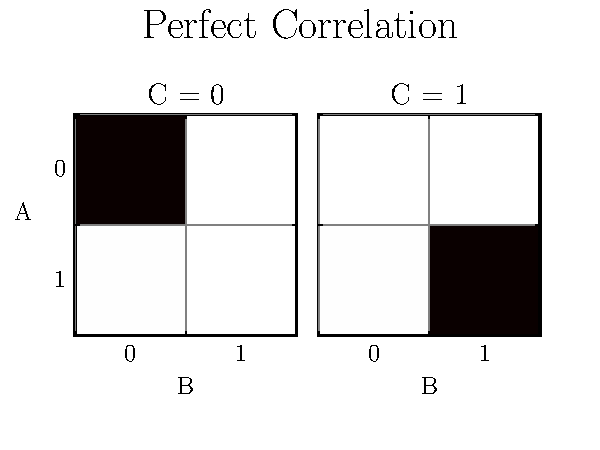
\includegraphics[width=\linewidth]{../../figures/distributions/perfect_correlation_2_outcomes.pdf}
        \end{center}
        \column{0.5\linewidth}
        \begin{align*}
        \probplotvalue{0, 0, 0} &= \f12 \\
        \prob[ABC][abc] &= \f{\bs{000} + \bs{111}}{2} \\
        \prob[ABC][abc] &= \begin{cases}
            \f12 & a = b = c \\
            0 & \text{ otherwise }
        \end{cases}
        \end{align*}
    \end{columns}
    \begin{center}
        Compatibility Inequality
    \end{center}
    \[ \prob[A][0]\prob[B][1] \leq \prob[BC][10] + \prob[AC][01] \]
    \begin{center}
        Witnesses Perfect Correlation
    \end{center}
    \[ \br{\f{1}{2}}^{2} \not\leq 0 + 0 \]
\end{frame}
\makeatletter
\renewcommand*\env@matrix[1][*\c@MaxMatrixCols c]{%
  \hskip -\arraycolsep
  \let\@ifnextchar\new@ifnextchar
  \array{#1}}
\makeatother
\begin{frame}
    \frametitle{Deriving Compatibility Inequalities}
    \begin{center}
        \scalebox{0.8}{\newcommand{\ift}{2.3}
\begin{tikzpicture}[scale=2]
    \begin{scope}[every node/.style=observed]
        \node (C1) at ({-2 + 3*1/\ift}, {3*1/(\ift*sqrt(3))}) {$\p{C}_1$};
        \node (B1) at ({2 - 3*1/\ift}, {3*1/(\ift*sqrt(3))}) {$\p{B}_1$};
        \node (A1) at (0, {2*sqrt(3) - 2*2/sqrt(3)*(1/\ift)}) {$\p{A}_1$};
    \end{scope}
    \begin{scope}[every node/.style=latent]
        \node (X1) at ({-1 + 1/\ift}, {sqrt(3) - 1/(\ift*sqrt(3))}) {$\p{X}_1$};
        \node (Y2) at (1, {sqrt(3)}) {$\p{Y}_2$};
        \node (Y1) at ({1 - 1/\ift}, {sqrt(3) - 1/(\ift*sqrt(3))}) {$\p{Y}_1$};
        \node (Z1) at (0, 0.5) {$\p{Z}_1$};
    \end{scope}
    \begin{scope}[every path/.style={draw=cause, thick}]
        \path[postaction={on each segment={mid arrow}}]
        (X1) -- (A1) (X1) -- (C1)
        (Y2) -- (A1) (Y1) -- (B1)
        (Z1) -- (B1) (Z1) -- (C1)
        ;
    \end{scope}
\end{tikzpicture}}
    \end{center}
    \[ \mscenario = \bc{\bc{A_1, B_1}, \bc{B_1, C_1}, \bc{A_1, C_1}} \]
    \[ \prob^{\mscenario} = \bc{\prob[A_1B_1], \prob[B_1C_1], \prob[A_1C_1]} \]
    \[ \text{Compatibility requires:} \qquad \exists \prob[\jointvar] = \prob[A_1B_1C_1] \]
    \[ \prob[A_1B_1] = {\sum}_{C_1} \prob[\jointvar] \qquad \prob[B_1C_1] = {\sum}_{A_1} \prob[\jointvar] \qquad \prob[A_1C_1] = {\sum}_{B_1} \prob[\jointvar]\]
\end{frame}

\begin{frame}[shrink=13]
    \frametitle{Deriving Compatibility Inequalities Cont'd}
    \[ \underbrace{\prob[A_1B_1] = {\sum}_{C_1} \prob[\jointvar] \qquad \prob[B_1C_1] = {\sum}_{A_1} \prob[\jointvar] \qquad \prob[A_1C_1] = {\sum}_{B_1} \prob[\jointvar]} \]
    \[ \underbrace{\forall V \in \mscenario: \prob[V] = \sum_{\jointvar \setminus V} \prob[\jointvar] }\]
    \[ \probvec^{\mscenario} = M \tcdot \probvec^{\jointvar}  \]
    \[ \probvec^{\mscenario} =
        \begin{pmatrix}
            \prob[A_1B_1][00] \\
            \prob[A_1B_1][01] \\
            \prob[A_1B_1][10] \\
            \prob[A_1B_1][11] \\
            \hline
            \prob[B_1C_1][00] \\
            \prob[B_1C_1][01] \\
            \prob[B_1C_1][10] \\
            \prob[B_1C_1][11] \\
            \hline
            \prob[A_1C_1][00] \\
            \prob[A_1C_1][01] \\
            \prob[A_1C_1][10] \\
            \prob[A_1C_1][11] \\
        \end{pmatrix}
        \qquad
        \probvec^{\jointvar} =
        \begin{pmatrix}
            \prob[A_1B_1C_1][000] \\
            \prob[A_1B_1C_1][001] \\
            \prob[A_1B_1C_1][010] \\
            \prob[A_1B_1C_1][011] \\
            \prob[A_1B_1C_1][100] \\
            \prob[A_1B_1C_1][101] \\
            \prob[A_1B_1C_1][110] \\
            \prob[A_1B_1C_1][111] \\
        \end{pmatrix}
    \]
\end{frame}

\begin{frame}[shrink=15]
    \frametitle{Incidence Example}
    \[ M = \kbordermatrix{
        (A_1,B_1,C_1) \:\: = & (0,0,0) & (0,0,1) & (0,1,0) & (0,1,1) & (1,0,0) & (1,0,1) & (1,1,0) & (1,1,1) \\
        (A_1=0, B_1=0) & \kone & \kone & \kzer & \kzer & \kzer & \kzer & \kzer & \kzer \\
        (A_1=0, B_1=1) & \kzer & \kzer & \kone & \kone & \kzer & \kzer & \kzer & \kzer \\
        (A_1=1, B_1=0) & \kzer & \kzer & \kzer & \kzer & \kone & \kone & \kzer & \kzer \\
        (A_1=1, B_1=1) & \kzer & \kzer & \kzer & \kzer & \kzer & \kzer & \kone & \kone \\
        (B_1=0, C_1=0) & \kone & \kzer & \kzer & \kzer & \kone & \kzer & \kzer & \kzer \\
        (B_1=0, C_1=1) & \kzer & \kone & \kzer & \kzer & \kzer & \kone & \kzer & \kzer \\
        (B_1=1, C_1=0) & \kzer & \kzer & \kone & \kzer & \kzer & \kzer & \kone & \kzer \\
        (B_1=1, C_1=1) & \kzer & \kzer & \kzer & \kone & \kzer & \kzer & \kzer & \kone \\
        (A_1=0, C_1=0) & \kone & \kzer & \kone & \kzer & \kzer & \kzer & \kzer & \kzer \\
        (A_1=0, C_1=1) & \kzer & \kone & \kzer & \kone & \kzer & \kzer & \kzer & \kzer \\
        (A_1=1, C_1=0) & \kzer & \kzer & \kzer & \kzer & \kone & \kzer & \kone & \kzer \\
        (A_1=1, C_1=1) & \kzer & \kzer & \kzer & \kzer & \kzer & \kone & \kzer & \kone
    } \]
    \[ \probvec^{\mscenario} = M \tcdot \probvec^{\jointvar}  \]
\end{frame}

\begin{frame}
    \frametitle{Marginal Linear Program}
    \begin{columns}[T]
        \column{0.4\linewidth}%
            \term{Marginal LP}:%
            \begin{alignat*}{2}
                & \text{minimize:} \quad&& \emptyset \tcdot x\\
                & \text{subject to:} && \probvec^{\jointvar} \succeq 0 \\
                & && M \tcdot \probvec^{\jointvar} = \probvec^{\mscenario} \\
            \end{alignat*}%
        \column{0.4\linewidth}%
            \term{Dual Marginal LP}:%
            \begin{alignat*}{2}
                & \text{minimize:} \quad&& y \tcdot \probvec^{\mscenario}\\
                & \text{subject to:} && y \tcdot M \succeq 0 \\
            \end{alignat*}%
    \end{columns}
    \begin{itemize}
        \item If $\probvec^{\jointvar}$ exists, then:
        \[ y \tcdot M \tcdot \probvec^{\jointvar} = y \tcdot \probvec^{\mscenario} \geq 0  \]
        \item If not, then $y$ is an \term{infeasibility certificate} which generates \term{infeasibility inequality}:
        \[ y \tcdot \probvec^{\mscenario} \geq 0 \]
        \item Most linear programing toolkits return certificates (\href[pdfnewwindow]{http://docs.mosek.com/8.0/pythonapi/optimizer-task-gety.html}{\textit{Mosek}}, \href[pdfnewwindow]{https://www.gurobi.com/documentation/6.5/refman/farkasdual.html}{\textit{Gurobi}}, \href[pdfnewwindow]{http://www-01.ibm.com/support/docview.wss?uid=swg21400058}{\textit{CPLEX}}, \href[pdfnewwindow]{http://cvxr.com/cvx/doc/basics.html\#dual-variables}{\textit{cvxr}}/\href[pdfnewwindow]{http://cvxopt.org/userguide/coneprog.html\#linear-cone-programs}{\textit{cvxopt}}.)
    \end{itemize}
    \note[item]{It is possible to derive non-contextuality inequalities from $M$ and a known incompatible distribution $\probvec^{\mscenario}$}
    \note[item]{Note the null objective; the minimization objective is trivially always zero}
    \note[item]{The primal value of the linear program is of no interest, all that matters is its \textit{feasibility}.}
    \note[item]{If \textit{feasible}, then there exists a vector $x$ that is a valid joint distribution vector $\probvec^{\jointvar}$.}
    \note[item]{Feasibility implies that $\probvec^{\jointvar} = x$.}
    \note[item]{Infeasibility implies contextuality}
\end{frame}


\begin{frame}
    \frametitle{Deflating Inequalities}
    \begin{columns}
        \column{0.5\linewidth}
            \scalebox{1.0}{\newcommand{\ift}{2.3}
\begin{tikzpicture}[scale=2]
    \begin{scope}[every node/.style=observed, onslide=<2->{fade}]
        \node (C1) at ({-2 + 3*1/\ift}, {3*1/(\ift*sqrt(3))}) {$\p{C}_1$};
        \node[onslide=<2->{unfade}] (B1) at ({2 - 3*1/\ift}, {3*1/(\ift*sqrt(3))}) {$\p{B}_1$};
        \node[onslide=<2->{unfade}] (A1) at (0, {2*sqrt(3) - 2*2/sqrt(3)*(1/\ift)}) {$\p{A}_1$};
    \end{scope}
    \begin{scope}[every node/.style=latent, onslide=<2->{fade}]
        \node[onslide=<2->{unfade}] (X1) at ({-1 + 1/\ift}, {sqrt(3) - 1/(\ift*sqrt(3))}) {$\p{X}_1$};
        \node[onslide=<2->{unfade}] (Y2) at (1, {sqrt(3)}) {$\p{Y}_2$};
        \node[onslide=<2->{unfade}] (Y1) at ({1 - 1/\ift}, {sqrt(3) - 1/(\ift*sqrt(3))}) {$\p{Y}_1$};
        \node[onslide=<2->{unfade}] (Z1) at (0, 0.5) {$\p{Z}_1$};
    \end{scope}
    \begin{scope}[every path/.style={draw=cause, thick}, onslide=<2->{fade}]
        \path[postaction={on each segment={mid arrow}}]
        (X1) -- (C1)
        (Z1) -- (C1)
        ;
        \path[postaction={on each segment={mid arrow}}, onslide=<2->{unfade}]
        (X1) -- (A1)
        (Y2) -- (A1)
        (Y1) -- (B1)
        (Z1) -- (B1)
        ;
    \end{scope}
\end{tikzpicture}}
        \column{0.5\linewidth}
            \vfill
            \begin{center}
            \[ \Inj[\graph]{\graph'} = \begin{Bmatrix}
                \bc{A_1,C_1}\\ \bc{B_1,C_1}\\ \bc{A_1}\\ \bc{B_1}\\ \bc{C_1}
            \end{Bmatrix} \]
            \[ \bc{A_1, B_1} \not \in \Inj[\graph]{\graph'} \]
            \end{center}
            \vfill
    \end{columns}
    \[ \prob[A_1B_1][01] \leq \prob[B_1C_1][10] + \prob[A_1C_1][01] \]
    \only<1>{\begin{center}\textbf{Can not deflate inequality!}\end{center}}
    \only<2>{\begin{center}\textbf{However!}\end{center}}
    \only<2>{\[ \AnSub[\graph']{A_1} \cap \AnSub[\graph']{B_1} = \emptyset \iff A_1 \ancestralindep B_1 \]}
    \onslide<3->{\[ \prob[A_1][0]\prob[B_1][1] \leq \prob[B_1C_1][10] + \prob[A_1C_1][01] \]}
    \onslide<4->{\[ \prob[A][0]\prob[B][1] \leq \prob[BC][10] + \prob[AC][01] \]}
\end{frame}

\begin{frame}
    \frametitle{Inflation Gives Polynomial Inequalities}
    \begin{itemize}
        \item Deflation only holds when inequality constrains probabilities $\prob[N'], N' \in \Inj[\graph]{\graph'}$
        \item \textbf{Linear inequality} for $\graph'$
    \end{itemize}
    \begin{center}
        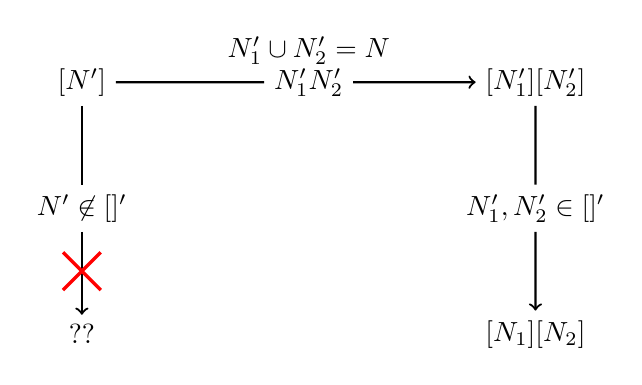
\begin{tikzpicture}[scale=0.8]
            \pgfmathsetmacro{\hs}{1.8};
            \pgfmathsetmacro{\vs}{1};
            \pgfmathsetmacro{\cross}{0.3};
            \draw (0*\hs, 4*\vs) node[](a){$\prob[N']$};
            \draw (0*\hs, 2*\vs) node[](ab){$N' \not \in \Inj[\graph]{\graph'}$};
            \draw (4*\hs, 4*\vs) node[](c){$\prob[N_1']\prob[N_2']$};
            \draw (2*\hs, 4*\vs) node[](ac){$N_1' \ancestralindep N_2'$};
            \draw (2*\hs, 4*\vs + 0.5*\vs) node[]{$N_1' \cup N_2' = N$};
            \draw (4*\hs, 2*\vs) node[](cd){$N_1', N_2' \in \Inj[\graph]{\graph'}$};
            \draw (4*\hs, 0*\vs) node[](d){$\prob[N_1]\prob[N_2]$};
            \draw (0, 0) node[](b){??};
            \draw[thick, ] (a) -- (ab);
            \draw[thick, ] (c) -- (cd);
            \draw[thick, ] (a) -- (ac);
            \draw[thick, ->] (ac) -- (c);
            \draw[thick, ->] (ab) -- (b);
            \draw[thick, ->] (cd) -- (d);
            \draw[very thick, red]
            (+ \cross, 1*\vs + \cross) -- (- \cross, 1*\vs - \cross)
            (+ \cross, 1*\vs - \cross) -- (- \cross, 1*\vs + \cross)
            ;
        \end{tikzpicture}
    \end{center}
    \begin{itemize}
        \item \textbf{Polynomial inequality} for $\graph$!
    \end{itemize}
\end{frame}

\begin{frame}
    \frametitle{Pre-injectable Sets}
    A \term{pre-injectable set} $N'$ is:
    \[ N' = {\coprod}_i N_i' \quad \forall i: N_i' \in \Inj[\graph]{\graph'} \]
    \[ \forall i, j : N_i' \ancestralindep N_j' \iff \An[\graph']{N'_i} \cap \An[\graph']{N'_j} = \emptyset \]
    Only need to consider \term{maximal pre-injectable sets} denoted $\PreInj[\graph]{\graph'}$
\end{frame}


\section{Appendix D: Quantum Non-classicality From Inflation}

\begin{frame}
    \frametitle{Triangle Scenario As Bell Scenario}
    \begin{center}
        \scalebox{1.0}{\begin{tikzpicture}[scale=1]
    \begin{scope}[every node/.style=observed]
        \node (C) at (0, -2.5) {$C$};
        \node (B) at (2, 2) {$B$};
        \node (A) at (-2, 2) {$A$};
    \end{scope}
    \begin{scope}[every node/.style=latent]
        \node (X) at (-2, 0) {$S_A$};
        \node (Y) at (0, 0.5) {$\la$};
        \node (Z) at (2, 0) {$S_B$};
    \end{scope}
    \begin{scope}[every path/.style={draw=cause, thick}]
        \path[postaction={on each segment={mid arrow}}]
        (X) -- (A)
        (X) -- (C)
        (Y) -- (A)
        (Y) -- (B)
        (Z) -- (B)
        (Z) -- (C);
    \end{scope}
\end{tikzpicture}}
    \end{center}
\end{frame}

\begin{frame}
    \frametitle{Fritz Distribution}
    \begin{center}
        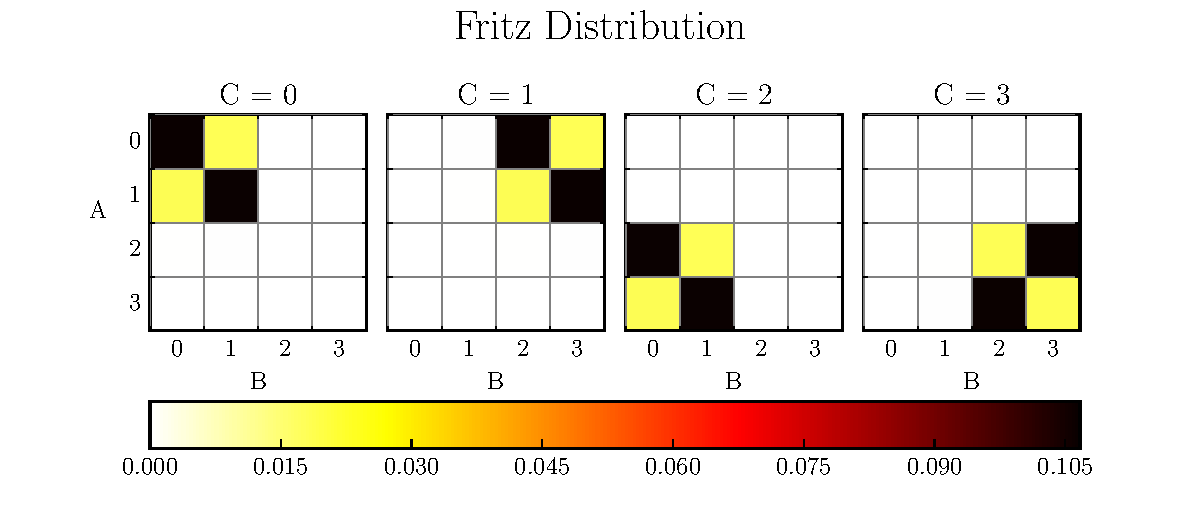
\includegraphics[width=\linewidth]{../../figures/distributions/fritz_dist_plot_brazil.pdf}
    \end{center}
    \[ \probplotvalue{253, 253, 84} = \f{1}{32}\br{2 - \sqrt{2}} \qquad \probplotvalue{11, 1, 0} = \f{1}{32}\br{2 + \sqrt{2}}\]
\end{frame}

\begin{frame}
    \frametitle{Fritz Distribution Bit-Measurements}
    \begin{center}
        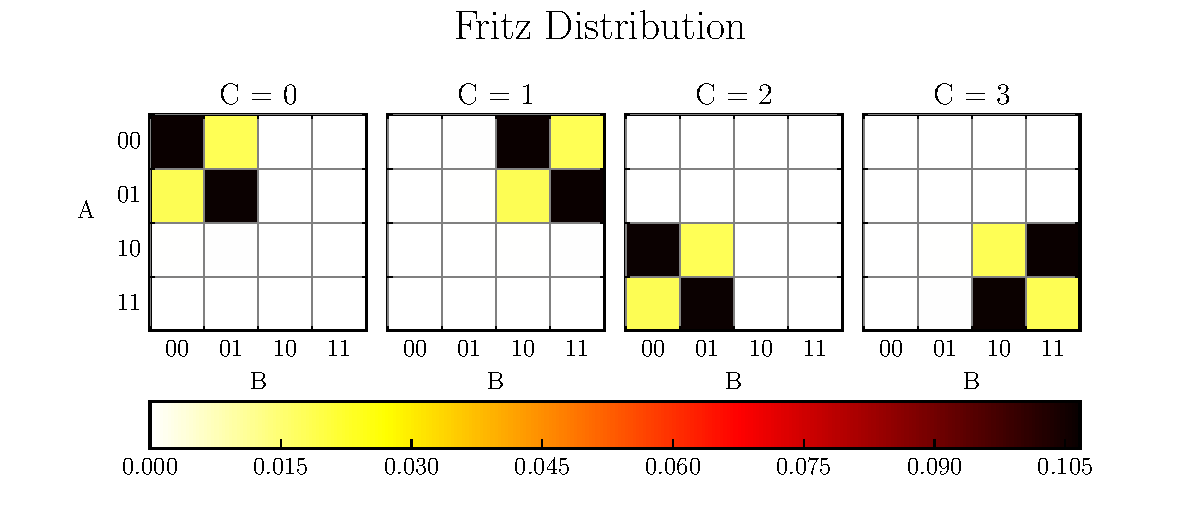
\includegraphics[width=\linewidth]{../../figures/distributions/fritz_dist_plot_bits_brazil.pdf}
    \end{center}
    \[ \probplotvalue{253, 253, 84} = \f{1}{32}\br{2 - \sqrt{2}} \qquad \probplotvalue{11, 1, 0} = \f{1}{32}\br{2 + \sqrt{2}}\]
\end{frame}

\begin{frame}
    \frametitle{Quantum Implementation of Fritz Distribution}
    \begin{itemize}
        \item States:
    \end{itemize}
    \begin{gather*}
        \rho_{AB} = \ket{\Phi^+}\bra{\Phi^+} \quad \rho_{BC} = \rho_{CA} = \f{\ket{00}\bra{00} + \ket{11}\bra{11}}{2}
    \end{gather*}
    \[ \ket{\Phi^+} = \f{1}{\sqrt{2}}\br{\ket{00} + \ket{11}} \]
    \begin{itemize}
        \item Measurements:
    \end{itemize}
    \begin{gather*}
        M_{A} = \bc{\ket{0\psi_{1}}\bra{0\psi_{1}}, \ket{0\psi_{5}}\bra{0\psi_{5}}, \ket{1\psi_{3}}\bra{1\psi_{3}}, \ket{1\psi_{7}}\bra{1\psi_{7}}} \\
        M_{B} = \bc{\ket{\psi_{6}0}\bra{\psi_{6}0}, \ket{\psi_{2}0}\bra{\psi_{2}0}, \ket{\psi_{0}1}\bra{\psi_{0}1}, \ket{\psi_{4}1}\bra{\psi_{4}1}} \\
        M_{C} = \bc{\ket{00}\bra{00}, \ket{10}\bra{10}, \ket{01}\bra{01}, \ket{11}\bra{11}}
    \end{gather*}
    \begin{itemize}
        \item Shorthand: $\ket{\psi_n} = \f{1}{\sqrt{2}}\br{\ket{0} + e^{in/4}\ket{1}}$
    \end{itemize}
\end{frame}

\begin{frame}
    \frametitle{Fritz Distribution Violating CHSH}
    % \begin{gather*}
    % \prob[F][00\textcolor{blue}{0}] = \prob[F][11\textcolor{blue}{0}] = \prob[F][30\textcolor{blue}{1}] = \prob[F][21\textcolor{blue}{1}] = \prob[F][12\textcolor{blue}{2}] = \prob[F][03\textcolor{blue}{2}] = \prob[F][23\textcolor{blue}{3}] = \prob[F][32\textcolor{blue}{3}] = \f{1}{32}\br{2 + \sqrt{2}} \\
    % \prob[F][01\textcolor{blue}{0}] = \prob[F][10\textcolor{blue}{0}] = \prob[F][31\textcolor{blue}{1}] = \prob[F][20\textcolor{blue}{1}] = \prob[F][13\textcolor{blue}{2}] = \prob[F][02\textcolor{blue}{2}] = \prob[F][22\textcolor{blue}{3}] = \prob[F][33\textcolor{blue}{3}] = \f{1}{32}\br{2 - \sqrt{2}}
    % \end{gather*}
    \begin{itemize}
        \item $C$'s outcome acts as measurement ``setting'' for A, B; independent of $\rho_{AB}$
        \item Correlation between right bits
    \end{itemize}
    \[ \ba{A_rB_r} = \prob[A_rB_r][00] + \prob[A_rB_r][11] - \prob[A_rB_r][01] - \prob[A_rB_r][10] \]
    \[ \ba{A_rB_r | C = 0, 1, 2} = \f{1}{\sqrt{2}} \quad \ba{A_rB_r | C = 3} = - \f{1}{\sqrt{2}} \]
    \begin{itemize}
        \item Gives CHSH violation
    \end{itemize}
    \begin{align*}
    &\ba{A_rB_r|C=0} + \ba{A_rB_r|C=1} + \ba{A_rB_r|C=2} - \ba{A_rB_r|C=3} \\
    &\quad = 3 \br{\f{1}{\sqrt{2}}} - \br{-\f{1}{\sqrt{2}}} \\
    &\quad = 2\sqrt{2} \not \leq 2
    \end{align*}
\end{frame}

\begin{frame}
    \frametitle{Notes on Fritz Distribution}
    \begin{itemize}
        \item Incompatibility proof contingent on perfect correlation between $C$ and pseudo-settings
        \item Proof not robust to noise
    \end{itemize}
    \begin{problem}[2.17 in \cite{Fritz_2012}]
        Find an example of non-classical quantum correlations in TS together with a proof of its non-classicality which does not hinge on Bell’s Theorem.
    \end{problem}
    \begin{itemize}
        \item ``...would be helpful to have inequalities...''
        % \item Possible to find inequalities violated by $\prob[F]$ using the Large inflation of the TS
    \end{itemize}
\end{frame}

\begin{frame}
    \frametitle{Large Inflation}
    \begin{center}
        \scalebox{1.0}{\newcommand{\ift}{2.3}
\begin{tikzpicture}[scale=2]
    \begin{scope}[every node/.style=observed]
        \node (C4) at (-2, 0) {$C_4$};
        \node (C3) at ({-2 + 1/\ift}, {1/(\ift*sqrt(3))}) {$C_3$};
        \node (C2) at ({-2 + 2*1/\ift}, {2*1/(\ift*sqrt(3))}) {$C_2$};
        \node (C1) at ({-2 + 3*1/\ift}, {3*1/(\ift*sqrt(3))}) {$C_1$};
        \node (B4) at (2, 0) {$B_4$};
        \node (B3) at ({2 - 1/\ift}, {1/(\ift*sqrt(3))}) {$B_3$};
        \node (B2) at ({2 - 2*1/\ift}, {2*1/(\ift*sqrt(3))}) {$B_2$};
        \node (B1) at ({2 - 3*1/\ift}, {3*1/(\ift*sqrt(3))}) {$B_1$};
        \node (A4) at (0, {2*sqrt(3)}) {$A_4$};
        \node (A3) at (0, {2*sqrt(3) - 2/sqrt(3)*(1/\ift)}) {$A_3$};
        \node (A2) at (0, {2*sqrt(3) - 2*2/sqrt(3)*(1/\ift)}) {$A_2$};
        \node (A1) at (0, {2*sqrt(3) - 3*2/sqrt(3)*(1/\ift)}) {$A_1$};
    \end{scope}
    \begin{scope}[every node/.style=latent]
        \node (X2) at (-1, {sqrt(3)}) {$X_2$};
        \node (X1) at ({-1 + 1/\ift}, {sqrt(3) - 1/(\ift*sqrt(3))}) {$X_1$};
        \node (Y2) at (1, {sqrt(3)}) {$Y_2$};
        \node (Y1) at ({1 - 1/\ift}, {sqrt(3) - 1/(\ift*sqrt(3))}) {$Y_1$};
        \node (Z1) at (0, 0.5) {$Z_1$};
        \node (Z2) at (0, 0) {$Z_2$};
    \end{scope}
    \begin{scope}[every path/.style={draw=cause, thick}]
        \path[postaction={on each segment={mid arrow}}]
        (X2) -- (A4) (X2) -- (C4) (X2) -- (C2) (X2) -- (A3)
        (Y2) -- (A4) (Y2) -- (B4) (Y2) -- (A2) (Y2) -- (B3)
        (Z2) -- (B4) (Z2) -- (C4) (Z2) -- (B2) (Z2) -- (C3)
        (X1) -- (A1) (X1) -- (C1) (X1) -- (C3) (X1) -- (A2)
        (Y1) -- (A1) (Y1) -- (B1) (Y1) -- (A3) (Y1) -- (B2)
        (Z1) -- (B1) (Z1) -- (C1) (Z1) -- (B3) (Z1) -- (C2)
        ;
    \end{scope}
\end{tikzpicture}}
    \end{center}
\end{frame}

\begin{frame}
    \frametitle{Large Inflation Pre-injectable Sets}
    \begin{equation*}
        \begin{gathered}
            \textbf{Maximal Pre-injectable Sets} \\
            \bc{A_1, B_1, C_1, A_4, B_4, C_4} \\
            \bc{A_1, B_2, C_3, A_4, B_3, C_2} \\
            \bc{A_2, B_3, C_1, A_3, B_2, C_4} \\
            \bc{A_2, B_4, C_3, A_3, B_1, C_2} \\
            \bc{A_1, B_3, C_4} \\
            \bc{A_1, B_4, C_2} \\
            \bc{A_2, B_1, C_4} \\
            \bc{A_2, B_2, C_2} \\
            \bc{A_3, B_3, C_3} \\
            \bc{A_3, B_4, C_1} \\
            \bc{A_4, B_1, C_3} \\
            \bc{A_4, B_2, C_1}
        \end{gathered}
        \qquad
        \begin{gathered}
            \textbf{Ancestral Independences} \\
            \bc{A_1, B_1, C_1} \ancestralindep \bc{A_4, B_4, C_4} \\
            \bc{A_1, B_2, C_3} \ancestralindep \bc{A_4, B_3, C_2} \\
            \bc{A_2, B_3, C_1} \ancestralindep \bc{A_3, B_2, C_4} \\
            \bc{A_2, B_4, C_3} \ancestralindep \bc{A_3, B_1, C_2} \\
            \bc{A_1} \ancestralindep \bc{B_3} \ancestralindep \bc{C_4} \\
            \bc{A_1} \ancestralindep \bc{B_4} \ancestralindep \bc{C_2} \\
            \bc{A_2} \ancestralindep \bc{B_1} \ancestralindep \bc{C_4} \\
            \bc{A_2} \ancestralindep \bc{B_2} \ancestralindep \bc{C_2} \\
            \bc{A_3} \ancestralindep \bc{B_3} \ancestralindep \bc{C_3} \\
            \bc{A_3} \ancestralindep \bc{B_4} \ancestralindep \bc{C_1} \\
            \bc{A_4} \ancestralindep \bc{B_1} \ancestralindep \bc{C_3} \\
            \bc{A_4} \ancestralindep \bc{B_2} \ancestralindep \bc{C_1}
        \end{gathered}
    \end{equation*}
\end{frame}

% \begin{frame}
%     \frametitle{Deriving Inequalities}
%     \begin{itemize}
%         \item Inflation facilitates turning linear, inflated inequalities into polynomial deflated ones
%         \item \textbf{Question:} How to derive compatibility inequalities for $\graph'$?
%         \item \textbf{Answer:} Use your favorite technique for deriving compatibility inequalities:
%         \begin{itemize}
%             \item Entropic inequalities
%             \item Finite outcome inequalities
%         \end{itemize}
%         \item Here we solve the marginal problem for $\mscenario = \PreInj[\graph]{\graph'}$
%         \item First some notation and formalism
%     \end{itemize}
% \end{frame}

\begin{frame}
    \frametitle{Large Inflation Incidence}
    \begin{itemize}
        \item Joint variables are all of the observable nodes $\nodes_O' = \jointvar$
        \[ \jointvar = \bc{A_1, A_2, A_3, A_4,B_1, B_2, B_3, B_4,C_1, C_2, C_3, C_4} \]
        \item Marginal scenario is composed of pre-injectable sets $\mscenario = \PreInj[\graph]{\graph'}$
        \item Inequalities violated by Fritz distribution are inherently $4$-outcome
        \item Incidence matrix $M$ is \textbf{very large} $\sim 2.25 \textsf{Gb}$
        \begin{itemize}
            \item $\# \text{Columns} = 4^{12} = 16,777,216$
            \item $\# \text{Rows} =  4\times 4^{6} + 8 \times 4^{3} = 16,896$
            \item $\# \text{Non-zero Entries} = 201,326,592$
        \end{itemize}
    \end{itemize}
\end{frame}

\section{Appendix F: Maximal Violations \& Noise}

\begin{frame}
    \frametitle{Numerical Optimization}
    Minimize objective function $f\br{\la} \in \R$:
    \begin{enumerate}
        \item Real-valued parameters $\la = \br{\la_0, \ldots, \la_n}$
        \item Quantum states/measurements $\rho_{AB}, \rho_{BC}, \rho_{CA}, M_{A}, M_{B}, M_{C}$
    \[ \prob[ABC]\br{abc} = \Tr\bs{\netperm^\intercal \rho_{AB}\otimes\rho_{BC}\otimes\rho_{CA} \netperm M_{A,a}\otimes M_{B,b} \otimes M_{C,c}} \]
        \item Distribution $\prob[ABC]$
        \item Plug into inequality $I$ in homogeneous form $I\br{\prob[ABC]} \geq 0$
        \item Output is objective value $I\br{\prob[ABC]}$
    \end{enumerate}
\end{frame}

\begin{frame}
    \frametitle{Numerical Optimization Methods}
    \begin{itemize}
        \item Numerical minimization of $f\br{\la}$
        \[ f(\la_{(k+1)}) = \la_{(k)} - \ga_{(k)} \del f(\la_{(k)})  \]
        \item Non-convex, non-linear, smooth/continuous
        \item Gradient Descent, BFGS Method, Nelder-Mead simplex method
        \item Stochastic methods: simulated annealing, basin-hopping
    \end{itemize}
\end{frame}

\begin{frame}
    \frametitle{Quantum Model On Triangle Scenario}
    \[ \prob[ABC]\br{abc} = \Tr\bs{\netperm^\intercal \rho_{AB}\otimes\rho_{BC}\otimes\rho_{CA} \netperm M_{A,a}\otimes M_{B,b} \otimes M_{C,c}} \]
    \begin{center}
        \scalebox{0.6}{\begin{tikzpicture}[scale=1]
    \begin{scope}[every node/.style=observed]
        \node (C) at (-2, 0) {$M_C$};
        \node (B) at (2, 0) {$M_B$};
        \node (A) at (0, {2*sqrt(3)}) {$M_A$};
    \end{scope}
    \begin{scope}[every node/.style=latent]
        \node (X) at (-1, {sqrt(3)}) {$\rho_{CA}$};
        \node (Y) at (1, {sqrt(3)}) {$\rho_{AB}$};
        \node (Z) at (0, 0) {$\rho_{BC}$};
    \end{scope}
    \begin{scope}[every path/.style={draw=cause, thick}]
        \path[postaction={on each segment={mid arrow}}]
        (X) -- (A)
        (X) -- (C)
        (Y) -- (A)
        (Y) -- (B)
        (Z) -- (B)
        (Z) -- (C);
    \end{scope}
\end{tikzpicture}}
    \end{center}
    \begin{itemize}
        \item Each latent resource $\rho \in \br{\rho_{AB}, \rho_{BC}, \rho_{CA}}$ modeled as bipartite \textbf{qubit} state acting on $\Hilb^{2} \otimes \Hilb^{2}$
        \item Each party $\br{A, B, C}$ is assigned $4$-outcome PVM set $\br{M_A, M_B, M_C}$
        \item Parameterized using unitary transformations $U \in \s{U}\br{4}$
    \end{itemize}
\end{frame}

\begin{frame}
    \frametitle{Parameterizing Unitary Group}
    \begin{itemize}
        \item \cite{Spengler_2010_Unitary} parameterization of $\s{U}\br{d}$
        \[ \la = \begin{pmatrix}
            \textcolor{Blue}{\la_{1,1}} & \textcolor{OliveGreen}{\cdots} & \textcolor{OliveGreen}{\la_{1, d}} \\
            \textcolor{Maroon}{\vdots} & \textcolor{Blue}{\ddots} & \textcolor{OliveGreen}{\vdots} \\
            \textcolor{Maroon}{\la_{d,1}} & \textcolor{Maroon}{\cdots} & \textcolor{Blue}{\la_{d, d}} \\
        \end{pmatrix} \]
        \[ U = \bs{\prod_{m=1}^{d-1} \br{\prod_{n=m+1}^{d} \textcolor{OliveGreen}{R_{m,n}} \textcolor{Maroon}{RP_{n,m}}}} \tcdot \bs{\prod_{l=1}^{d} \textcolor{Blue}{GP_{l}}} \]
        \item Global Phase Terms: \textcolor{Blue}{$GP_{l} = \exp\br{iP_l \lambda_{l,l}}$}
        \item Relative Phase Terms: \textcolor{Maroon}{$RP_{n,m} = \exp\br{i P_n \lambda_{n,m}}$}
        \item Rotation Terms: \textcolor{OliveGreen}{$R_{m,n} = \exp\br{i \si_{m,n} \lambda_{m,n}}$}
        \item Projection Operators: $P_l = \ket{l}\bra{l}$
        \item Anti-symmetric $\si$-matrices: $\si_{m,n} = - i\ket{m}\bra{n} + i \ket{n}\bra{m}$
        \item Parameters $\la_{n,m} \in \bs{0, 2\pi}$
    \end{itemize}
\end{frame}

\begin{frame}
    \frametitle{Parameterizing Unitary Group Cont'd}
    \begin{itemize}
        \item Each parameter $\la_{n,m}$ has physical interpretation
        \item Degeneracies are easily eliminated such as global phase
        \[ \forall l = 1, \ldots, d : \la_{l,l} = 0 \implies GP_{l} = \ident \]
        \item Parameterize $U \in \s{U}\br{d}$ up to global phase denoted $\ti{U} \in \s{U}\br{d}$
        % \[ \ti{U}_{k} = \prod_{m=1}^{k} \br{\prod_{n={m+1}}^{d} R_{m,n} RP_{n,m}} \]
        \[ \ti{U} = \prod_{m=1}^{d} \br{\prod_{n={m+1}}^{d} R_{m,n} RP_{n,m}} \]
        \item Computationally efficient (no matrix exponentials)
        \begin{alignat*}{2}
            GP_l &= \ident &&+ P_l \br{e^{i\la_{l,l}} - 1} \\
            RP_{n,m} &= \ident &&+ P_n \br{e^{i\la_{n,m}} - 1} \\
            R_{m,n} &= \ident &&+ \br{\ket{m}\bra{m} + \ket{n}\bra{n}} \br{\cos\lambda_{n,m} - 1} \\
            & &&+ \br{\ket{m}\bra{n} - \ket{n}\bra{m}} \sin\lambda_{n,m} \\
        \end{alignat*}
    \end{itemize}
\end{frame}

\begin{frame}
    \frametitle{Parameterizing PVMs}
    \begin{itemize}
        \item Each part is assigned $d$ element \term{projective-valued measures (PVMs)} acting on $\s{H}^d$,
        \[ M = \bc{M_1, \ldots, M_d} \qquad \sum_{i=1}^{d} M_{i} = \ident \]
        \[ \forall i: \forall \ket{\psi} \in \Hilb^d : \bra{\psi} M_i \ket{\psi} \geq 0 \quad M_i = M_i^{\dagger} \]
        \[ M_{i}M_{j} = \de_{ij} M_{i} \quad M_{i} = \ket{m_{i}}\bra{m_{i}} \]
        % \item Inspired by \cite{Pal_2010}, parameterizing PVMs means parameterizing a $n$-element sub-basis $\bc{\ket{m_{\chi,i}}}$
        \item Unitary transform maps $M$ to computational basis
        \[ \bc{\ket{m_{1}}, \ldots, \ket{m_{d}}} = \bc{U \ket{1}, \ldots, U \ket{d}} \]
        \item Global phase irrelevant: $\ti{U}$ requires $d(d - 1)$ real-valued parameters
        \item PVMs are computationally more efficient than POVMs
    \end{itemize}
    \[ \prob[ABC]\br{abc} = \bra{m_{A,a}m_{B,b}m_{C,c}}{\netperm^\intercal \rho_{AB}\otimes\rho_{BC}\otimes\rho_{CA} \netperm}\ket{m_{A,a}m_{B,b}m_{C,c}} \]
\end{frame}

\begin{frame}
    \frametitle{Parameterizing States}
    \begin{itemize}
        \item Exploit spectral decomposition
        \[ \rho = \sum_{i=1}^{d} p_i \ket{\psi_i} \bra{\psi_i} \qquad p_i \geq 0, \sum_i p_i = 1 \]
        \item Unitary transform maps $\bc{\ket{\psi_i}}$ to computational basis
        \[ \bc{\ket{\psi_{1}}, \ldots, \ket{\psi_{d}}} = \bc{U \ket{1}, \ldots, U \ket{d}} \]
        \item Global phase irrelevant again $\ti{U}$ requires $d\br{d - 1}$ real-valued parameters
        \item Eigenvalues $\bc{p_i}$ parameterized using hyper-spherical coordinates: $d - 1$ real-valued parameters
    \end{itemize}
\end{frame}

\begin{frame}
    \frametitle{Maximal Violation}
    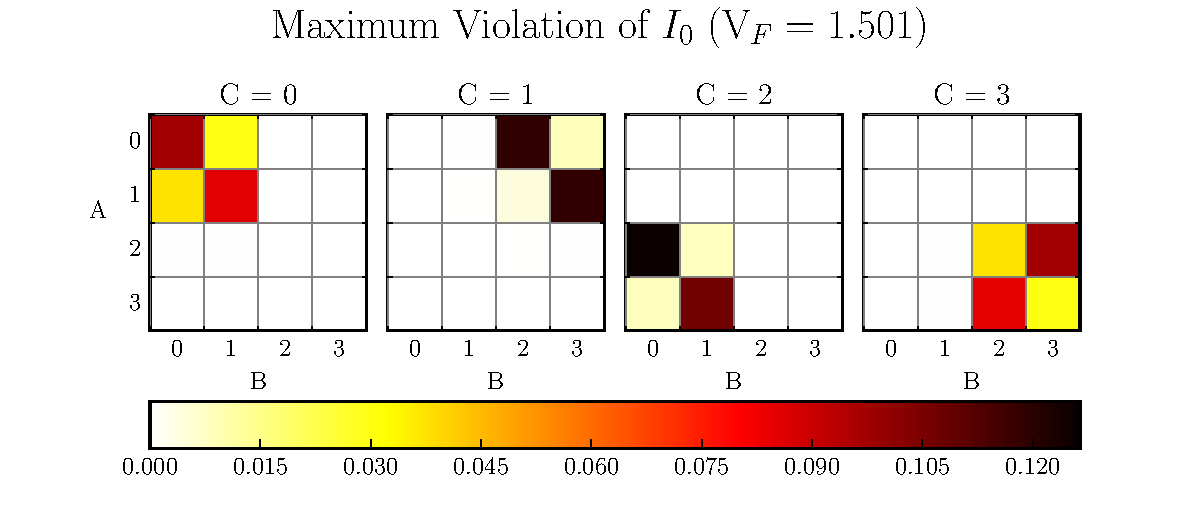
\includegraphics[width=\linewidth]{../../figures/distributions/plotted_dist_I_0_max_violation.pdf}
    \[ \text{Relative Violation:} \qquad V_F = \f{\min_P\bc{I\br{P}}}{I\br{P_F}} \]
\end{frame}

\begin{frame}
    \frametitle{Maximal Violation Symmetric}
    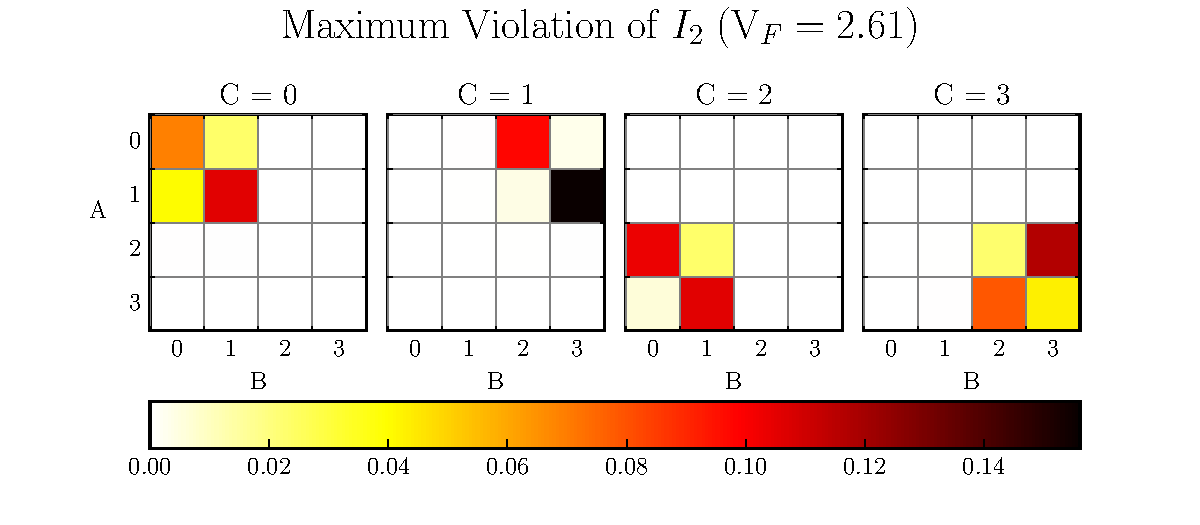
\includegraphics[width=\linewidth]{../../figures/distributions/plotted_dist_I_2_max_violation.pdf}
    \[ \text{Relative Violation:} \qquad V_F = \f{\min_P\bc{I\br{P}}}{I\br{P_F}} \]
\end{frame}

\begin{frame}
    \frametitle{Max Entangled vs. Max Violating} % $\chi = -2$
    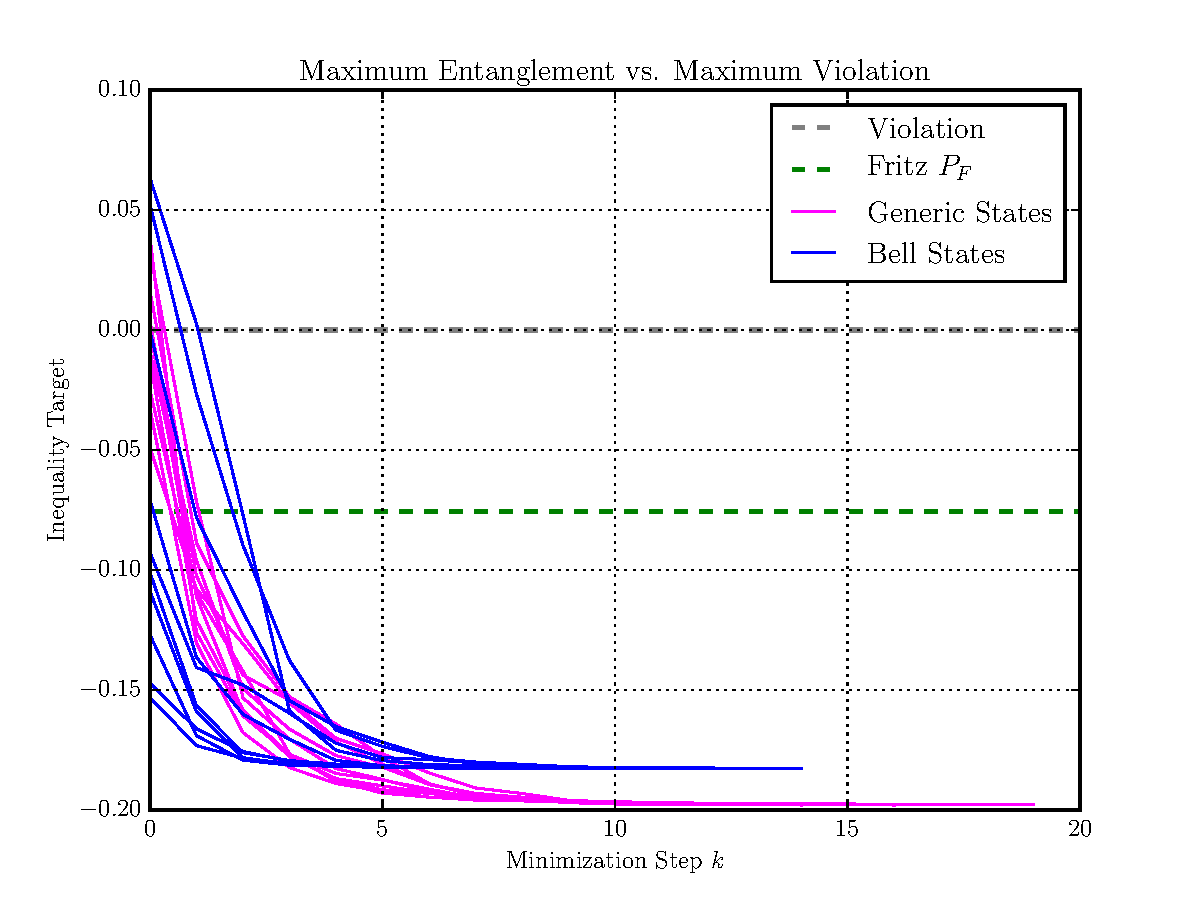
\includegraphics[width=\linewidth]{../../figures/optimizations/Max_Entanglement_vs_Max_Violation_fritz_seed.pdf}
\end{frame}

\begin{frame}
    \frametitle{Maximally Violating Distributions}
    \begin{itemize}
        \item Able to out-perform violation provided by Fritz distribution
        \item Maximally-violating states are not maximally-entangled; similar to detection loop-hole example of \cite{Methot_2006}
        \item Both symmetric and asymmetric inequalities exhibit same qualitative features
        % \item Violation very sensitive to the initial parameters $\la_{(0)}$
    \end{itemize}
\end{frame}
\begin{frame}
    \frametitle{Uniform Noise}
    \[ \s{U}_{\varepsilon}\br{P} = \br{1 - \varepsilon} P + \varepsilon \s{U} \]
    \begin{center}
        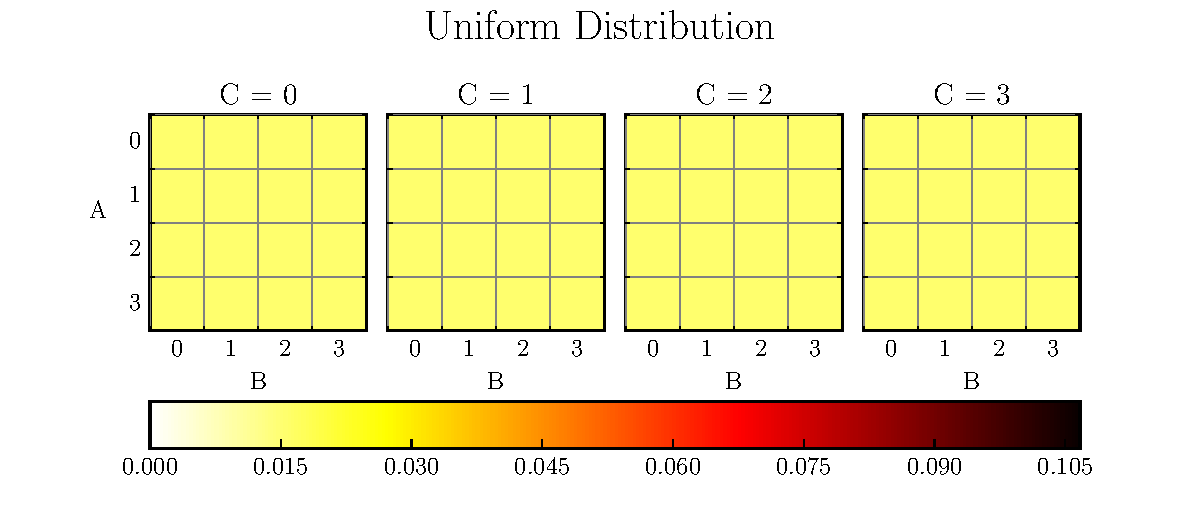
\includegraphics[width=\linewidth]{../../figures/distributions/uniform_dist_plot.pdf}
    \end{center}
    \[ \probplotvalue{255, 255, 109} = \f{1}{64} \]
    % \begin{center}
    %     \begin{tikzpicture}
    %         \pgfmathsetmacro{\ts}{0.5}; % term spacing
    %         \draw[] (0*\ts,0) node[]{$P_\varepsilon$};
    %         \draw[] (1*\ts,0) node[]{$=$};
    %         \draw[] (2*\ts,0) node[]{$(1-\varepsilon)P_{F}$};
    %         \draw[] (3*\ts,0) node[]{$+$};
    %         \draw[] (4*\ts,0) node[]{$\delta$};
    %     \end{tikzpicture}
    % \end{center}
\end{frame}

\begin{frame}
    \frametitle{Robust to Noise}
    \begin{center}
        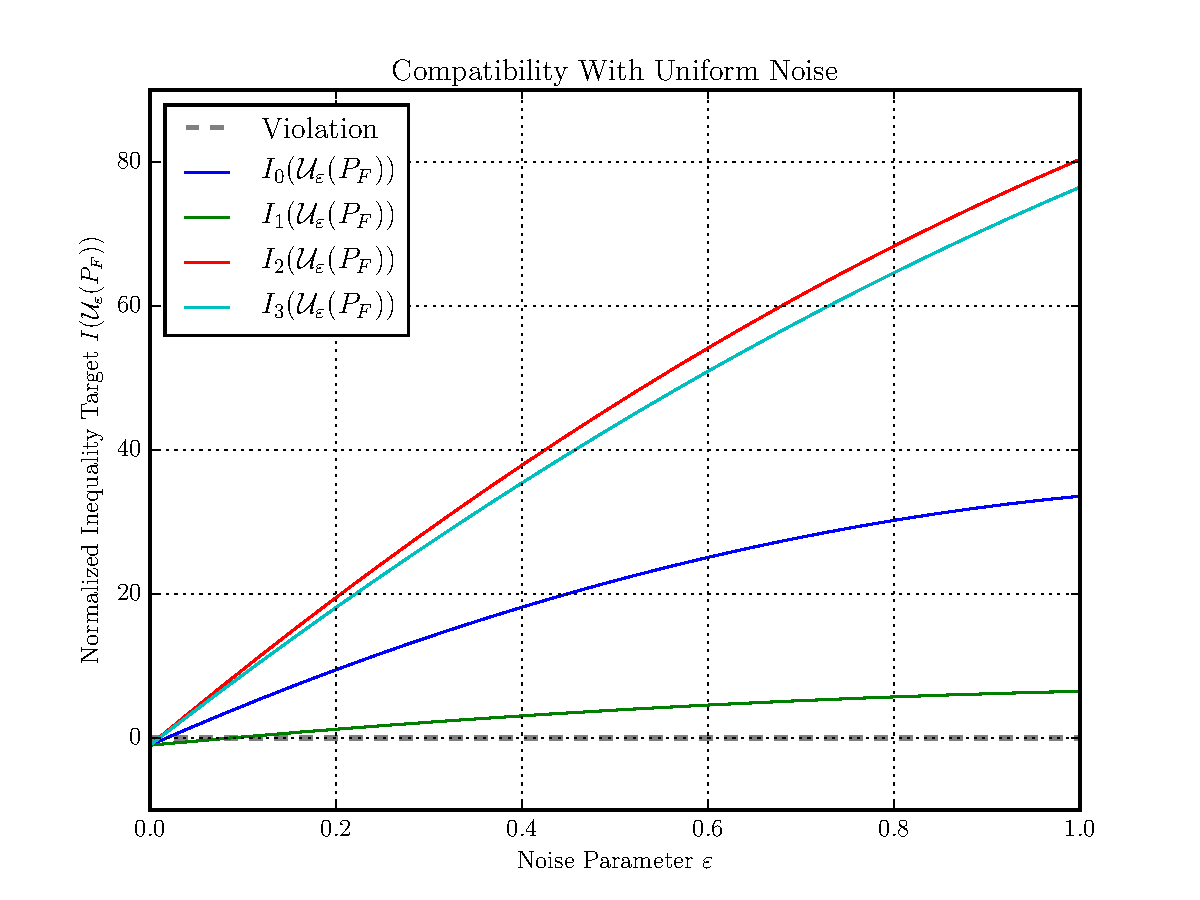
\includegraphics[width=\linewidth]{../../figures/noise/four_rep_inequalities_uniform_noise.pdf}
    \end{center}
\end{frame}

\begin{frame}
    \frametitle{Robust to Noise Zoomed}
    \begin{center}
        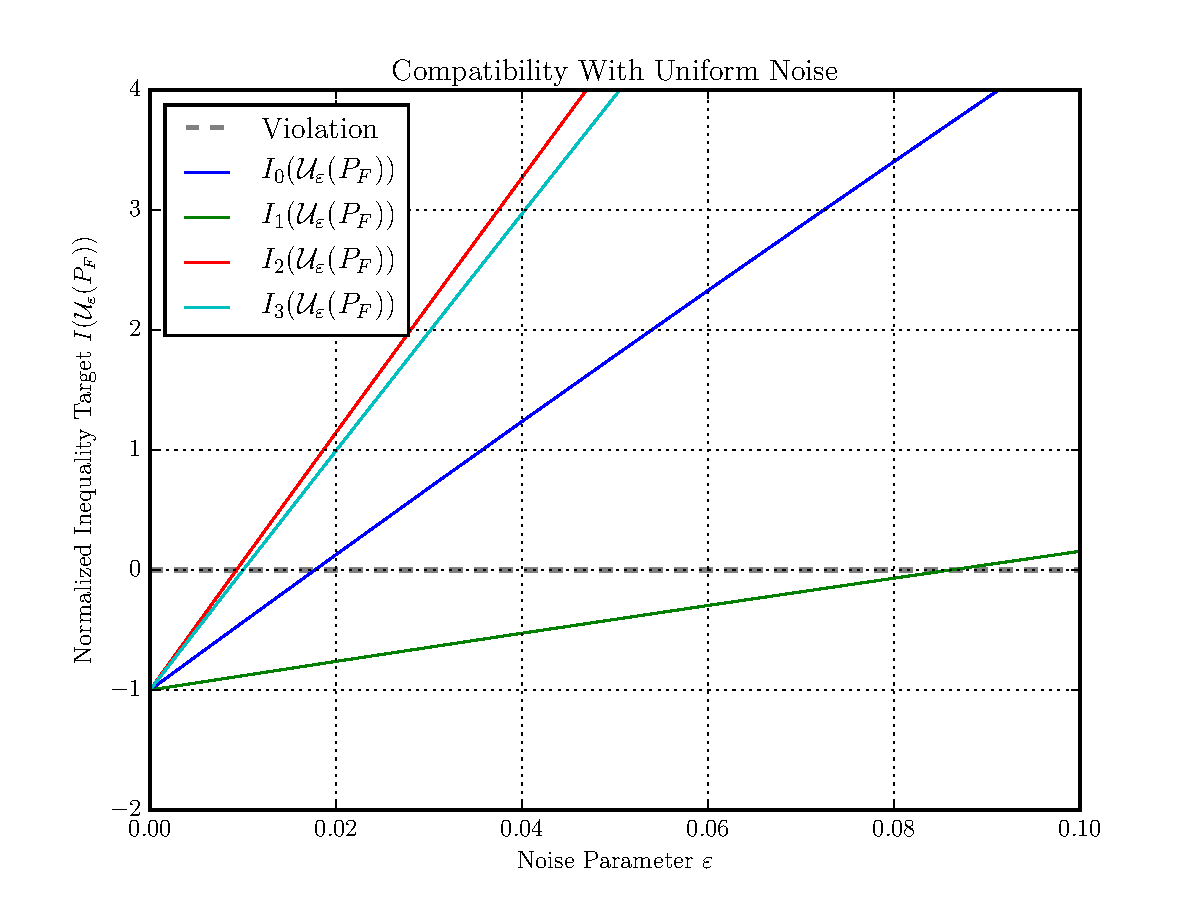
\includegraphics[width=\linewidth]{../../figures/noise/four_rep_inequalities_uniform_noise_zoomed.pdf}
    \end{center}
\end{frame}

\begin{frame}
    \frametitle{Noisy Non-locality}
    \begin{center}
        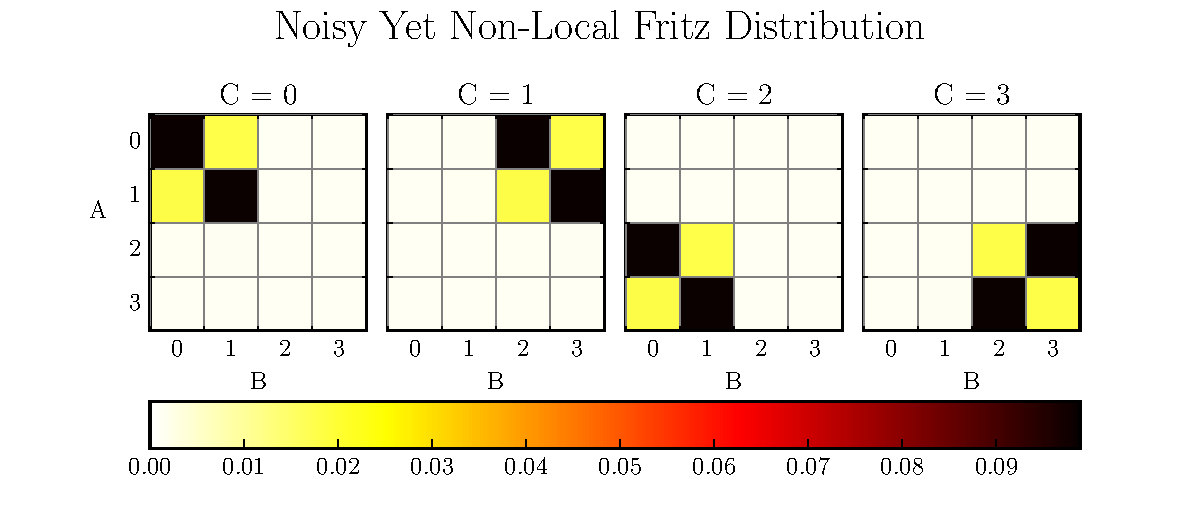
\includegraphics[width=\linewidth]{../../figures/noise/noisy_yet_non_local_fritz.pdf}
    \end{center}
    \[ \probplotvalue{255, 255, 243} = 0.00133 \]
\end{frame}

\begin{frame}
    \frametitle{Conclusions}
    \begin{enumerate}
        \item \textbf{Inflation technique} capable of producing polynomial inequalities with quantum/classical witnesses
        \item Fritz witness-able by \textbf{party-symmetric inequalities}
        \item Maximally violating distributions require \textbf{non-maximally entangled states}
    \end{enumerate}
\end{frame}

\begin{frame}
    \frametitle{Unanswered Questions}
    \begin{enumerate}
        \item Do these new non-local distributions suggest \textbf{new quantum resources} in the triangle scenario?
        \item Can any non-local quantum correlations in the triangle scenario \textbf{satisfy CHSH inequalities} (under Fritz type coarse graining)?
        \item Which inequalities are \textbf{most robust} to noise? Facets?
    \end{enumerate}
\end{frame}

% \begin{frame}
%     \frametitle{Postdoc Opportunities At The Perimeter Institute}
%     \begin{center}
%     \textbf{Two Postdoctoral Fellowships in Quantum Foundations at the Perimeter Institute} \\
%     Project: \textit{Quantum Causal Structures} \\
%     \vfill
%     \begin{itemize}
%         \item How to define quantum causal models
%         \item Quantum causal inference
%         \item How to provide causal explanations of Bell inequality violations
%         \item Exploring the possibilities for indefinite causal structure
%     \end{itemize}
%     \vfill
%     {\scriptsize Application \& Info:}\\

%     The Perimeter Website $\to$ Research $\to$ Careers $\to$ Positions $\to$ Quantum Causal Structures Postdoctoral Fellowship
%     \textcolor{blue}{\url{https://www.perimeterinstitute.ca/2016/17-quantum-causal-structures-postdoctoral-fellowship}}
%     \vfill

%     {\scriptsize Funded by the John Templeton Foundation}
%     \end{center}

% \end{frame}
\end{document}